\documentclass[pdflatex,sn-mathphys-num]{sn-jnl}

\usepackage{graphicx}
\usepackage{multirow}
\usepackage{amsmath,amssymb,amsfonts}
\usepackage{amsthm}
\usepackage{mathrsfs}
\usepackage[title]{appendix}
\usepackage{xcolor}
\usepackage{textcomp}
\usepackage{manyfoot}
\usepackage{booktabs}
\usepackage{array}
\usepackage{url}

\graphicspath{{figures/}}

\theoremstyle{thmstyleone}
\newtheorem{theorem}{Theorem}
\newtheorem{proposition}{Proposition}

\newcommand{\SplitSlab}{\textsc{SplitSlab}}
\newcommand{\RecallBench}{\textsc{RecallRegret-Bench}}
\newcommand{\RoPE}{\mathrm{RoPE}}
\newcommand{\WAF}{\mathrm{WAF}}
\newcommand{\E}{\mathbb{E}}

\raggedbottom

\begin{document}

\title[SplitSlab: Write-Once Split-Plane KV-Cache Tiering]{SplitSlab: Write-Once Split-Plane KV-Cache Tiering for Low Write Amplification and Delayed Recall in LLM Serving}

\author*[1]{\fnm{Mohammed Kamran} \sur{Syed}}\email{mohammedkamran.syed@ieee.org}
\author[2]{\fnm{Anudeep} \sur{Rentala}}\email{anudeep.rentala@ieee.org}
\author[2]{\fnm{Somesh} \sur{Rahul}}\email{someshrahul@ieee.org}
\author[3]{\fnm{Raghuram Malpe} \sur{Pai}}\email{raghuram.pai@ieee.org}
\author[3]{\fnm{Krishna Suman} \sur{Dara}}\email{krishna-suman.dara@ieee.org}

\affil*[1]{\orgname{Independent Researcher}, \orgaddress{\city{Mountain House}, \state{CA}, \postcode{95391}, \country{USA}}}
\affil[2]{\orgname{Independent Researcher}, \orgaddress{\city{Fremont}, \state{CA}, \postcode{94538}, \country{USA}}}
\affil[3]{\orgname{Independent Researcher}, \orgaddress{\city{Sunnyvale}, \state{CA}, \postcode{94086}, \country{USA}}}

\abstract{Long-running Large Language Model (LLM) agents often combine two memory optimizations: online Key-Value (KV) eviction in GPU High-Bandwidth Memory (HBM) and content-addressed KV offloading to NVMe Solid-State Drives (SSDs). Putting these two techniques together breaks three important properties of flash storage and multi-turn inference. First, when different agents ask different questions about a shared prompt, query-driven eviction keeps different tokens for each agent and drops cross-agent SHA-256 block sharing from 100\% to 0\%. Second, re-compacting older KV blocks on every turn rewrites flash pages repeatedly and causes 7.5$\times$ to 53.7$\times$ NVMe write amplification. Third, permanently deleting low-attention tokens causes compaction regret when a later turn asks about an early detail that was never queried before. We present \SplitSlab{}, a write-once two-plane KV tiering engine that resolves these three issues. \SplitSlab{} splits each finished prefix block once, using only deterministic prefix rules, into a 20\% hot HBM anchor skeleton and an exact 64\,KB cold NVMe residual stripe, while keeping a 64-byte bias-centered subspace sketch in HBM. During decoding, a parameter-free two-layer lookahead query scores upcoming cold sketches and streams needed stripes from NVMe during normal layer execution whenever output entropy and sketch prominence cross a threshold. Across four 3\,B to 14\,B Qwen2.5 and Granite models on a unified-memory workstation prototype with uncached direct NVMe I/O (\texttt{F\_NOCACHE}), \SplitSlab{} keeps NVMe write amplification at 1.00$\times$, preserves 100\% cross-agent deduplication, cuts steady HBM usage by 77.4\% to 79.6\%, and recovers up to 95.0\% delayed-recall accuracy while reading fewer than 7\% of cold stripes.}

\keywords{KV-cache tiering, NVMe write amplification, Large language model serving, Content-addressed deduplication, Subspace routing sketches, Memory-storage co-design}

\maketitle

% ============================================================================
\section{Introduction}\label{sec:intro}
% ============================================================================

Multi-turn LLM agents for software engineering, incident response, and repository analysis routinely process conversations spanning tens of thousands of tokens~\cite{jimenez2024swebench,zheng2024sglang}. Because attention Key-Value (KV) memory grows linearly with sequence length and batch size, serving systems usually combine two techniques to stay within GPU High-Bandwidth Memory (HBM) limits. The first technique is online KV compaction, such as \texttt{H2O}~\cite{zhang2023h2o}, \texttt{StreamingLLM}~\cite{xiao2024streamingllm}, and \texttt{SnapKV}~\cite{li2024snapkv}, which keeps about 20\% of high-attention tokens in HBM and drops the rest. The second technique is NVMe KV offloading, such as \texttt{vLLM}~\cite{kwon2023vllm}, \texttt{DistServe}~\cite{zhong2024distserve}, \texttt{CacheGen}~\cite{liu2024cachegen}, \texttt{Mooncake}~\cite{qin2025mooncake}, and \texttt{LMCache}~\cite{cheng2025lmcache}, which saves KV blocks to flash storage indexed by the SHA-256 hash of the uncompacted token prefix~\cite{quinlan2002venti}.

Combining query-driven eviction with content-addressed NVMe storage creates three direct system failures at the GPU-flash boundary:

\begin{enumerate}
  \item \emph{Prefix-Hash Collapse (0\% Fleet Sharing).} Suppose Agents A and B load the same repository snapshot in Turn~1. In Turn~2, Agent A inspects an ingress router module while Agent B inspects an OpenTelemetry exporter. Online policies like \texttt{SnapKV} and \texttt{H2O} score Turn~1 tokens using each agent's Turn~2 queries. The surviving token lists diverge inside the very first block, shifting every later block boundary and dropping cross-agent SHA-256 block deduplication from 100\% to 0.0\%. In our 32-agent fleet test on \texttt{Qwen2.5-7B}, query-driven eviction writes 287.00\,MB to flash, which is 4.43$\times$ more than storing the full uncompacted KV cache (64.75\,MB).

  \item \emph{Flash Write Amplification (7.5$\times$ to 53.7$\times$ WAF).} NVMe SSDs and Zoned Namespaces (ZNS)~\cite{hu2009waf,bjorling2021zns,rosenblum1992lfs} achieve their best speed and lifespan when software writes aligned 64\,KB stripes once and never modifies them. Re-compacting KV state across $K$ turns removes different tokens from older blocks on each turn, forcing repeated 64\,KB read-modify-write cycles. In our measurements, this raises physical write amplification ($\WAF$) to 7.54$\times$--20.13$\times$ across 12 to 24 turns, and up to 53.67$\times$ when writes use unaligned 24\,KB chunks.

  \item \emph{Compaction Regret on Delayed Recall.} Early background facts, such as an unused error constant (\texttt{LEGACY\_RENEG\_ABORT\_HEX = 0x7F3A}), get very low attention during unrelated middle turns (Turns~3 to 11) and are permanently deleted. When a crash dump in Turn~12 asks about \texttt{0x7F3A}, irreversible eviction baselines score 0.0\% exact match across all 72 multi-model runs in our benchmark.
\end{enumerate}

Existing recallable KV systems solve only part of this problem. \texttt{Quest}~\cite{tang2024quest} skips attention work using bounding boxes, but it keeps 100\% of KV pages in GPU HBM and saves no GPU memory. Host-DRAM offloaders such as \texttt{FlexGen}~\cite{sheng2023flexgen}, \texttt{InfiniGen}~\cite{lee2024infinigen}, \texttt{ArkVale}~\cite{chen2024arkvale}, \texttt{ShadowKV}~\cite{sun2025shadowkv}, and \texttt{RetrievalAttention}~\cite{liu2024retrievalattention} rely on local CPU DRAM, build query-dependent or per-head layouts that break fleet SHA-256 sharing, or wait until Layer~$\ell$ to fetch pages synchronously, which stalls decoding on 70 to 190\,$\mu\mathrm{s}$ NVMe reads.

We design and implement \SplitSlab{}, a write-once split-plane KV storage and speculative recall engine built for GPU HBM compaction and direct NVMe flash tiering (Fig.~\ref{fig:arch}). \SplitSlab{} keeps global prefix hashing intact while letting the GPU drop 80\% of historical KV state from HBM without losing the ability to recover it later. This paper makes four contributions:

\begin{enumerate}
  \item \emph{Zero-Padding 64\,KB Split-Plane Layout ($\WAF = 1.00\times$).} We derive a block sizing rule for Grouped-Query Attention (GQA)~\cite{ainslie2023gqa} that maps standard KV head counts $H_{\mathrm{kv}} \in \{2, 4, 8\}$ (at head size $d_h = 128$, FP16) to logical block lengths $M \in \{80, 40, 20\}$. The evicted 80\% residual slice fills exactly 65,536 bytes (64.0\,KB) per layer with zero padding. Because the split uses only prefix tokens and fixed stride rules, collaborating agents produce byte-identical hot skeletons and cold NVMe stripes, giving 100.0\% SHA-256 deduplication and $\WAF = 1.00\times$.

  \item \emph{64-Byte Bias-Centered Routing Sketch (1,024$\times$ Compression).} Each 64\,KB cold stripe leaves a tiny 64-byte binary sketch $S_{m,\ell}$ in HBM (0.098\% overhead). The sketch stores $C=2$ salience-weighted sub-cluster sign projections~\cite{charikar2002simhash,gao2024rabitq} across 240 static $W_Q/W_K$ directions plus two FP16 norms. Before sketching, \SplitSlab{} subtracts the deterministic Rotary Position Embedding (RoPE)~\cite{su2024roformer} key-projection bias (whose norm reaches 920.5 in \texttt{Qwen2.5}~\cite{yang2024qwen25}) and co-routes resident Plane-0 anchors so tokens split across planes are still found.

  \item \emph{Parameter-Free Two-Layer Speculative Lookahead.} Scoring Layer~$\ell$ queries $q_t^{(\ell)}$ directly against Layer~$\ell+2$ key sketches fails (0.0102 cosine similarity and 0.0\% recall) because each layer uses its own head basis. Projecting the Layer~$\ell$ residual state through Layer~$\ell+2$'s existing RMSNorm and $W_Q^{(\ell+2)}$ weights raises cosine similarity to 0.9623 with zero trained parameters. This lets \SplitSlab{} overlap 72.7 to 189.1\,$\mu\mathrm{s}$ uncached NVMe reads inside 2.03 to 5.17\,ms two-layer compute windows.

  \item \emph{Formal Bounds and Multi-Model Uncached NVMe Evaluation.} We prove a non-asymptotic attention output bound $\|O_{\SplitSlab} - O_{\mathrm{FullKV}}\|_2 \le 2 \alpha_{\mathcal{R}} \max_i \|V_i\|_2$ (checked with zero violations across 560 real attention heads), a greedy token preservation condition, and linear $\Omega(K)$ write amplification bounds for re-compaction. Across \texttt{Qwen2.5-3B}, \texttt{Qwen2.5-7B}, \texttt{Granite-3.1-8B}~\cite{mishra2024granite}, and \texttt{Qwen2.5-Coder-14B} using Darwin \texttt{F\_NOCACHE} uncached NVMe reads, \SplitSlab{} saves 77.4\% to 79.6\% of steady GPU HBM and recovers 45.0\% to 95.0\% exact delayed recall (55.0\% to 95.0\% field accuracy), while online eviction scores 0.0\%.
\end{enumerate}

\begin{figure*}[t]
\centering
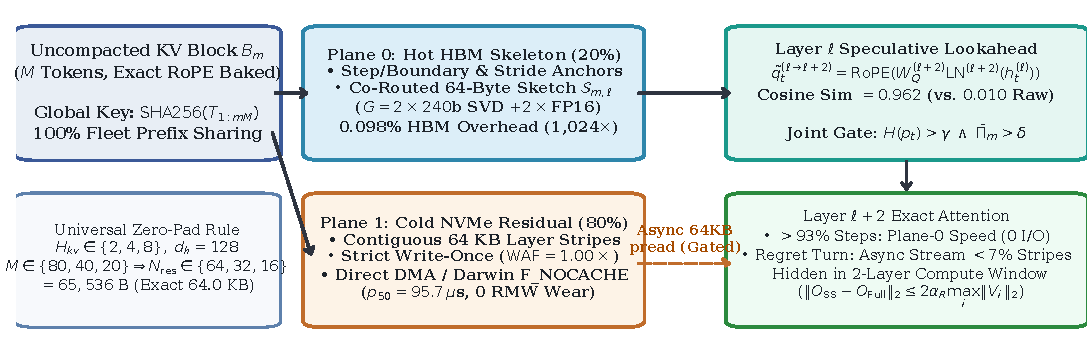
\includegraphics[width=\textwidth]{fig1_architecture_overview.pdf}
\caption{Overview of the \SplitSlab{} two-plane storage architecture and asynchronous recall pipeline. Completed prefix blocks $B_m$ ($M \in \{80, 40, 20\}$ tokens for $H_{\mathrm{kv}} \in \{2, 4, 8\}$) split deterministically from prefix tokens alone into a 20\% Plane-0 HBM skeleton and an exact 65,536-byte (64.0\,KB) write-once Plane-1 NVMe stripe ($\WAF = 1.00\times$, 100\% SHA-256 sharing). Each cold stripe leaves a 64-byte bias-centered sketch $S_{m,\ell}$ in HBM. At Layer~$\ell$, a parameter-free speculative query $\tilde{q}_t^{(\ell\to\ell+2)}$ scores Layer~$\ell+2$ sketches and streams needed 64\,KB stripes inside the two-layer compute window whenever predictive entropy $H(p_t) > \gamma$ and block prominence $\bar{\Pi}_m > \delta$.}
\label{fig:arch}
\end{figure*}

The rest of this paper is organized as follows. Section~\ref{sec:related} compares \SplitSlab{} with prior KV-cache eviction, sparse attention, and offloading engines. Section~\ref{sec:arch} describes the split-plane layout, 64-byte sketch, and two-layer lookahead gate. Section~\ref{sec:theory} presents our formal bounds with plain-English intuition (full proofs are in Appendix~\ref{app:proofs}). Section~\ref{sec:methodology} explains our uncached NVMe prototype, models, and benchmark. Section~\ref{sec:eval} reports experimental results, ablations, and baseline comparisons. Section~\ref{sec:limits} discusses practical limitations, and Section~\ref{sec:conclusion} concludes.

% ============================================================================
\section{Background and Related Work}\label{sec:related}
% ============================================================================

Table~\ref{tab:prior_art} compares \SplitSlab{} against six families of KV-cache systems across HBM savings, delayed recall, storage alignment, flash write amplification, prefix deduplication, and prefetching.

\begin{table*}[t]
\centering
\caption{Comparison of KV-cache eviction, sparse attention, CPU offloading, and direct NVMe storage systems.}
\label{tab:prior_art}
\footnotesize
\renewcommand{\arraystretch}{1.15}
\setlength{\tabcolsep}{4pt}
\resizebox{\textwidth}{!}{%
\begin{tabular}{@{}lcccccc@{}}
\toprule
\textbf{System / Paradigm} & \textbf{GPU HBM} & \textbf{Delayed-Recall} & \textbf{Offload Tier \&} & \textbf{Flash} & \textbf{Cross-Agent} & \textbf{Zero-Param Async} \\
 & \textbf{Savings} & \textbf{Recovery} & \textbf{Page Alignment} & $\mathbf{\WAF}$ & \textbf{SHA-256 Dedup} & \textbf{NVMe Lookahead} \\
\midrule
\texttt{vLLM}~\cite{kwon2023vllm}, \texttt{Mooncake}~\cite{qin2025mooncake}, \texttt{LMCache}~\cite{cheng2025lmcache} & $0\%$ & Yes ($100\%$) & NVMe / RDMA ($64$\,KB+) & $1.00\times$ & Yes ($100\%$) & N/A (Full HBM) \\
\texttt{H2O}~\cite{zhang2023h2o}, \texttt{StreamingLLM}~\cite{xiao2024streamingllm}, \texttt{SnapKV}~\cite{li2024snapkv} & $75\%$--$80\%$ & No ($0\%$) & None (Irreversible Drop) & N/A & No ($0\%$) & No \\
Online Evict + Naive NVMe Re-Compaction & $75\%$--$80\%$ & No ($0\%$) & Ragged / Mutable SSD & $7.5\times$--$53.7\times$ & No ($0\%$) & No \\
\texttt{Quest}~\cite{tang2024quest} (HBM Bounding-Box Skip) & $0\%$ & Yes & None ($100\%$ in HBM) & N/A & Yes & No (Sync Layer $\ell$) \\
\texttt{ArkVale}~\cite{chen2024arkvale}, \texttt{ShadowKV}~\cite{sun2025shadowkv}, \texttt{RetrievalAttn}~\cite{liu2024retrievalattention} & $70\%$--$83\%$ & Yes & Local CPU DRAM Only & Unaligned & No (Per-Head/Idx) & No (Sync Layer $\ell$) \\
\texttt{InfiniGen}~\cite{lee2024infinigen} (Skewed CPU Prefetch) & $60\%$--$75\%$ & Partial & Local CPU DRAM Only & Unaligned & No & Requires Trained $A^{(\ell)}$ \\
\midrule
\textbf{\SplitSlab{} (Ours)} & $\mathbf{77.4\%\text{--}79.6\%}$ & \textbf{Yes ($\mathbf{95\%}$ 7B)} & \textbf{Direct NVMe (Exact 64\,KB)} & $\mathbf{1.00\times}$ & \textbf{Yes ($\mathbf{100\%}$)} & \textbf{Yes ($\tilde{q}_t^{(\ell\to\ell+2)}$, 0 Params)} \\
\bottomrule
\end{tabular}%
}
\end{table*}

\subsection{Content-Addressed KV Pools}
Serving engines such as \texttt{vLLM}~\cite{kwon2023vllm} and \texttt{SGLang}~\cite{zheng2024sglang} manage fixed-size KV blocks in GPU HBM and share common system prompts or codebases via prefix hashes. Systems like \texttt{DistServe}~\cite{zhong2024distserve}, \texttt{CacheGen}~\cite{liu2024cachegen}, \texttt{Mooncake}~\cite{qin2025mooncake}, and \texttt{LMCache}~\cite{cheng2025lmcache} extend this idea to cluster-wide DRAM and NVMe pools~\cite{quinlan2002venti}. However, these systems store uncompacted blocks. Every active request must load 100\% of its prefix back into GPU HBM during decoding, so HBM capacity remains the bottleneck on long multi-turn sessions.

\subsection{Irreversible Online KV Eviction and Flash WAF}
\texttt{StreamingLLM}~\cite{xiao2024streamingllm} keeps initial sink tokens plus a sliding window, \texttt{H2O}~\cite{zhang2023h2o} keeps cumulative heavy-hitter tokens, and \texttt{SnapKV}~\cite{li2024snapkv} selects prompt tokens using an observation window of recent queries. These methods work well for single-turn summarization, where one query defines what matters. In multi-turn agent workflows, however, permanent eviction drops background tokens that later turns need. Pairing query-driven eviction with SSD storage also breaks log-structured and zoned flash design rules~\cite{rosenblum1992lfs,hu2009waf,bjorling2021zns}: query-specific token lists break cross-agent SHA-256 sharing, and re-compacting old blocks on every turn rewrites flash pages over and over.

\subsection{Sparse Attention and CPU DRAM Offloading}
\texttt{Quest}~\cite{tang2024quest} stores coordinate-wise $[k_{\min}, k_{\max}]$ bounding boxes per KV page to skip \texttt{FlashAttention}~\cite{dao2022flashattention} tiles, yet keeps 100\% of KV tensors in GPU HBM (using 16\,KB of metadata per page on top of full page storage). \texttt{FlexGen}~\cite{sheng2023flexgen}, \texttt{ArkVale}~\cite{chen2024arkvale}, \texttt{ShadowKV}~\cite{sun2025shadowkv}, and \texttt{RetrievalAttention}~\cite{liu2024retrievalattention} offload evicted pages, low-rank values, or vector indexes to node-local CPU DRAM. Host DRAM is much smaller and costlier per gigabyte than NVMe flash, per-head page divergence breaks cross-agent content hashing, and synchronous Layer~$\ell$ recall stalls decoding across 70 to 190\,$\mu\mathrm{s}$ NVMe reads. \texttt{InfiniGen}~\cite{lee2024infinigen} overlaps CPU transfers with one layer of prefetching, but it needs offline-trained skewing matrices $A^{(\ell)}$ for every model and keeps dense partial keys in host memory. \SplitSlab{} needs no auxiliary training, keeps $\WAF = 1.00\times$ on direct NVMe flash, preserves 100\% fleet deduplication, and hides NVMe latency using two-layer lookahead.

% ============================================================================
\section{SplitSlab Architecture}\label{sec:arch}
% ============================================================================

Consider a Grouped-Query Attention (GQA)~\cite{ainslie2023gqa} transformer with $L$ decoder layers, $H_q$ query heads, $H_{\mathrm{kv}}$ key-value heads ($G_{\mathrm{gqa}} = H_q / H_{\mathrm{kv}}$ query heads per KV group), and head dimension $d_h$. For token position $p \in \mathbb{N}_0$ in Layer~$\ell \in \{0,\dots,L-1\}$, the post-$\RoPE$ key and value tensors $k_p^{(\ell)}, v_p^{(\ell)} \in \mathbb{F}_{16}^{H_{\mathrm{kv}} \times d_h}$ take $b_{\mathrm{tok}} = 4 H_{\mathrm{kv}} d_h$ bytes per token per layer (2 bytes per FP16 value across both $K$ and $V$).

\subsection{Zero-Padding 64\,KB Split-Plane Layout}\label{subsec:layout}

NVMe SSDs, GPUDirect Storage (\texttt{GDS}), and ZNS zones perform best when writes are sequential, immutable, and aligned to $P_{\mathrm{flash}} = 65{,}536$ bytes (64.0\,KB), avoiding sub-page read-modify-write penalties and internal flash garbage collection~\cite{hu2009waf,bjorling2021zns}. Given a target hot HBM anchor ratio $\rho \in (0,1)$ (default $\rho = 0.20$) and an uncompacted recent window $W_{\mathrm{loc}}$ (default 48 tokens), \SplitSlab{} picks the logical block size $M$ so that the evicted $(1-\rho)$ slice of each layer block equals $P_{\mathrm{flash}}$ bytes with zero wasted space:
\begin{equation}\label{eq:stripe_rule}
N_{\mathrm{res}} = \frac{P_{\mathrm{flash}}}{4 H_{\mathrm{kv}} d_h}, \quad
N_{\mathrm{anc}} = \left\lfloor \frac{\rho}{1-\rho} N_{\mathrm{res}} + \frac{1}{2} \right\rfloor, \quad
M = N_{\mathrm{anc}} + N_{\mathrm{res}}.
\end{equation}

Table~\ref{tab:geometry} applies~\eqref{eq:stripe_rule} to all four models we evaluate. Zero padding holds whenever $b_{\mathrm{tok}} = 4 H_{\mathrm{kv}} d_h$ divides $65{,}536$, which covers every standard power-of-two GQA head count $H_{\mathrm{kv}} \in \{1, 2, 4, 8, 16\}$ at $d_h = 128$ FP16 (and FP8 KV caches as well, where $b_{\mathrm{tok}} = 2 H_{\mathrm{kv}} d_h$ simply doubles $N_{\mathrm{res}}$). For non-power-of-two head counts such as $H_{\mathrm{kv}} = 6$, setting $N_{\mathrm{res}} = \lfloor P_{\mathrm{flash}} / b_{\mathrm{tok}} \rfloor$ packs 21 tokens with 2.3\% zero-tail padding while keeping $\WAF = 1.00\times$.

\begin{table}[t]
\centering
\caption{Zero-padding 64.0\,KB stripe geometry ($d_h = 128$, $\rho = 0.20$) and measured two-layer decode compute windows on our testbed.}
\label{tab:geometry}
\footnotesize
\renewcommand{\arraystretch}{1.15}
\setlength{\tabcolsep}{6pt}
\begin{tabular}{@{}lcccccc@{}}
\toprule
\textbf{Model ($H_q{:}H_{\mathrm{kv}}$)} & $L$ & $b_{\mathrm{tok}}$ & $M$ & $N_{\mathrm{anc}}$ / $N_{\mathrm{res}}$ & \textbf{Stripe Size} & \textbf{2-Layer Window} \\
\midrule
\texttt{Qwen2.5-3B} ($16{:}2$) & $36$ & $1$\,KB & $80$ & $16$ / $64$ & $65{,}536$\,B & $2{,}033.8\,\mu\mathrm{s}$ \\
\texttt{Qwen2.5-7B} ($28{:}4$) & $28$ & $2$\,KB & $40$ & $8$ / $32$ & $65{,}536$\,B & $4{,}813.1\,\mu\mathrm{s}$ \\
\texttt{Granite-8B} ($32{:}8$) & $40$ & $4$\,KB & $20$ & $4$ / $16$ & $65{,}536$\,B & $4{,}087.7\,\mu\mathrm{s}$ \\
\texttt{Qwen2.5-14B} ($40{:}8$) & $48$ & $4$\,KB & $20$ & $4$ / $16$ & $65{,}536$\,B & $5{,}167.3\,\mu\mathrm{s}$ \\
\bottomrule
\end{tabular}
\end{table}

Once logical block $B_m = \{mM, \dots, (m+1)M - 1\}$ moves behind the recent window $W_{\mathrm{loc}}$, \SplitSlab{} assigns it a global content hash from the uncompacted prefix tokens alone:
\begin{equation}\label{eq:canon_hash}
h_m = \operatorname{SHA256}\!\big(t_0, t_1, \dots, t_{(m+1)M-1}\big).
\end{equation}
It then splits $B_m$ into two disjoint index sets $B_m = B_m^{(0)} \sqcup B_m^{(1)}$ ($|B_m^{(0)}| = N_{\mathrm{anc}}$ and $|B_m^{(1)}| = N_{\mathrm{res}}$) using a fixed, query-free rule:
\begin{enumerate}
  \item \emph{Plane~0 (Hot HBM Anchor Skeleton).} \SplitSlab{} ranks positions inside $B_m$ by a deterministic priority tuple $(\text{tier}, -\text{rel\_pos})$: first, the opening $\max(1, N_{\mathrm{anc}}/4)$ sink slots (tier~100); second, chat or role boundary tokens $\mathcal{V}_{\mathrm{bound}}$ (tier~50, earliest position wins ties); and third, evenly spaced stride slots ($i \bmod \lfloor M/N_{\mathrm{anc}} \rfloor = 0$, tier~10). It takes the top $N_{\mathrm{anc}}$ slots, which cleanly handles tight blocks like $M = 20, N_{\mathrm{anc}} = 4$ even when sinks and boundary tokens together exceed four slots. Every kept key retains its original baked $\RoPE$ position $p \in B_m^{(0)}$.
  \item \emph{Plane~1 (Cold NVMe Residual Stripe).} \SplitSlab{} packs the remaining $N_{\mathrm{res}}$ keys and values for Layer~$\ell$ into one contiguous 65,536-byte stripe $\Sigma_{m,\ell} = [\operatorname{vec}(K_{B_m^{(1)}}^{(\ell)}) \,\|\, \operatorname{vec}(V_{B_m^{(1)}}^{(\ell)})]$. If $(h_m, \ell)$ is not yet in the content-addressed NVMe store, it writes $\Sigma_{m,\ell}$ once at a 64\,KB-aligned offset.
\end{enumerate}

Because $B_m^{(0)}$, $B_m^{(1)}$, and $h_m$ depend only on prefix tokens $t_{0:(m+1)M-1}$, any two agents sharing a prefix up to block $m$ build identical Plane-0 skeletons and share the exact same $(h_m, \ell)$ NVMe stripes with zero duplicate flash writes.

\subsection{Bias-Centered 64-Byte Subspace Routing Sketch}\label{subsec:sketch}

To know which evicted Plane-1 stripe to fetch without keeping full keys in DRAM, \SplitSlab{} stores a compact 64-byte sketch $S_{m,\ell}$ in HBM for every 64\,KB stripe (1,024$\times$ compression, or 0.098\% HBM overhead).

\subsubsection{Removing Pre-RoPE Key-Projection Bias}
Models such as \texttt{Qwen2.5}~\cite{yang2024qwen25} add a learned key-projection bias $b_K^{(\ell)} \in \mathbb{R}^{H_{\mathrm{kv}} d_h}$ before applying rotary embeddings:
\begin{equation}\label{eq:rope_bias}
k_p^{(\ell)} = \RoPE\!\big(W_K^{(\ell)}\,\mathrm{RMSNorm}(h_p^{(\ell)}),\, p\big) + \RoPE\!\big(b_K^{(\ell)},\, p\big).
\end{equation}
Across \texttt{Qwen2.5-7B}'s 28 layers, $\|b_K^{(\ell)}\|_2$ ranges from 11.4 to 920.5 (mean 85.4). Because $\RoPE(b_K^{(\ell)}, p)$ rotates with token position $p$, averaging raw keys over a block produces a loud sinusoidal bias wave that drowns out token meaning. Before building a sketch (and on HBM reference keys during scoring), \SplitSlab{} subtracts the known bias term $\RoPE(b_K^{(\ell)}, p)$ to isolate the content vector $\mathring{k}_p^{(\ell)} = k_p^{(\ell)} - \RoPE(b_K^{(\ell)}, p)$. This step needs no queries and costs almost nothing. On bias-free models like \texttt{Granite-3.1-8B}~\cite{mishra2024granite}, $b_K^{(\ell)} = 0$ so $\mathring{k}_p^{(\ell)} = k_p^{(\ell)}$.

\subsubsection{Sub-Cluster Centroids and 1-Bit Packing}
Averaging all $N_{\mathrm{res}}$ cold tokens into a single vector dilutes short literals such as a 5-token hex error code (\texttt{0x7F3A}). Instead, \SplitSlab{} splits $B_m^{(1)}$ into $C = 2$ contiguous halves $B_{m,1}^{(1)}$ and $B_{m,2}^{(1)}$ of $N_{\mathrm{res}}/2$ tokens each. Inside each half $c \in \{1, 2\}$ and KV head $g \in \{1, \dots, H_{\mathrm{kv}}\}$, it computes a norm-weighted centroid:
\begin{equation}\label{eq:salience_centroid}
\mu_{m,c,g}^{(\ell)} = \sum_{p \in B_{m,c}^{(1)}} w_{p,g}\,\mathring{k}_{p,g}^{(\ell)}, \quad
w_{p,g} = \frac{\exp(\eta\|\mathring{k}_{p,g}^{(\ell)}\|_2)}{\sum_{p' \in B_{m,c}^{(1)}} \exp(\eta\|\mathring{k}_{p',g}^{(\ell)}\|_2)},
\end{equation}
with $\eta = 0.35$. Moderate norm weighting lifts rare identifiers and hex codes without letting a single outlier token dominate the centroid.

At model load time, \SplitSlab{} computes a fixed orthonormal subspace $P_{\ell,g} \in \mathbb{R}^{d_h \times d_{\mathrm{sub}}}$ ($d_{\mathrm{sub}} = 240 / H_{\mathrm{kv}}$, giving $d_{\mathrm{sub}} \in \{120, 60, 30\}$ for $H_{\mathrm{kv}} \in \{2, 4, 8\}$) directly from the model's pretrained weights. Specifically, let $\Sigma_{K,g}^{(\ell)} = W_{K,g}^{(\ell)} W_{K,g}^{(\ell)\top}$ and $\Sigma_{Q,g}^{(\ell)} = \frac{1}{G_{\mathrm{gqa}}} \sum_{r=1}^{G_{\mathrm{gqa}}} W_{Q,g,r}^{(\ell)} W_{Q,g,r}^{(\ell)\top}$ be the $d_h \times d_h$ key and query covariance matrices (summing outer products across query heads prevents sign cancellation), and let $\psi_j = \big|\frac{2}{N_{\mathrm{res}}} \sum_{u=0}^{N_{\mathrm{res}}/2 - 1} e^{i u \theta_j}\big|$ measure how well rotary plane $j$ stays phase-aligned across a sub-cluster. The columns of $P_{\ell,g}$ are the top-$d_{\mathrm{sub}}$ eigenvectors of $\mathrm{diag}(\psi)(\Sigma_{K,g}^{(\ell)} \Sigma_{Q,g}^{(\ell)} + \Sigma_{Q,g}^{(\ell)} \Sigma_{K,g}^{(\ell)})\mathrm{diag}(\psi)$.

Projecting $z_{m,c,g}^{(\ell)} = P_{\ell,g}^\top \mu_{m,c,g}^{(\ell)} \in \mathbb{R}^{d_{\mathrm{sub}}}$ and concatenating across all $H_{\mathrm{kv}}$ heads yields a 240-dimensional vector $z_{m,c}^{(\ell)}$ per sub-cluster. Using asymmetric 1-bit quantization~\cite{charikar2002simhash,gao2024rabitq}, we store:
\begin{equation}\label{eq:sketch_pack}
S_{m,\ell} = \Big(
\underbrace{\|z_{m,1}^{(\ell)}\|_2^{\mathbb{F}_{16}},\, \|z_{m,2}^{(\ell)}\|_2^{\mathbb{F}_{16}}}_{4\text{ bytes } (2 \times \mathrm{FP16})},\;
\underbrace{\operatorname{sign}(z_{m,1}^{(\ell)}),\, \operatorname{sign}(z_{m,2}^{(\ell)})}_{480\text{ bits} = 60\text{ bytes}}
\Big),
\end{equation}
which takes exactly 64 bytes per 64\,KB stripe across every GQA configuration.

\subsection{Basis-Aligned Lookahead and Co-Routed Recall Gate}\label{subsec:lookahead}

\subsubsection{Two-Layer Speculative Query Projection}
To hide a 70 to 190\,$\mu\mathrm{s}$ uncached NVMe read, Layer~$\ell$ must start prefetching stripes for Layer~$\ell + \Delta\ell$ ($\Delta\ell = 2$ by default). Scoring Layer~$\ell$'s own query $q_t^{(\ell)}$ directly against Layer~$\ell+\Delta\ell$'s key sketches fails because $W_Q^{(\ell)}$ and $W_K^{(\ell+\Delta\ell)}$ live in different head coordinate systems. However, in Pre-LN transformers the residual stream changes gradually between nearby layers ($h_t^{(\ell+\Delta\ell)} = h_t^{(\ell+1)} + \sum_{u=\ell+1}^{\ell+\Delta\ell-1} \Delta h_t^{(u)}$, and in $\mu\text{P}$ models like \texttt{Granite-3.1-8B} each step is scaled by 0.22). \SplitSlab{} therefore projects the current Layer~$\ell$ output state $h_t^{(\ell+1)}$ through Layer~$\ell+\Delta\ell$'s own static RMSNorm and query matrix $W_Q^{(\ell+\Delta\ell)}$:
\begin{equation}\label{eq:spec_query}
\tilde{q}_t^{(\ell \to \ell+\Delta\ell)} = \RoPE\!\Big(W_Q^{(\ell+\Delta\ell)}\,\mathrm{RMSNorm}^{(\ell+\Delta\ell)}\!\big(h_t^{(\ell+1)}\big),\, p_t\Big).
\end{equation}
This single-token projection costs $O(d_{\mathrm{model}}^2)$ FLOPs, does not grow with context length $T$, uses zero extra parameters, and places $\tilde{q}_t^{(\ell\to\ell+\Delta\ell)}$ in Layer~$\ell+\Delta\ell$'s exact coordinate basis.

\subsubsection{Co-Routed Plane-0 Beacon and Prominence Scoring}
Let $\hat{z}_{m,c}^{(\ell')}$ be the unit-variance vector decoded from sketch $S_{m,\ell'}$ and zero-centered across cold blocks $m \in \{1, \dots, M_{\mathrm{cold}} - R_{\mathrm{rec}}\}$ (where $R_{\mathrm{rec}} = \lceil 240/M \rceil$ skips blocks right next to $W_{\mathrm{loc}}$). For a scaled speculative query $\tilde{q}$ (using $s_{\mathrm{attn}} = 1/\sqrt{d_h}$, or $1/d_h$ under $\mu\text{P}$), the estimated Plane-1 logit on block $m$ is:
\begin{equation}\label{eq:sketch_logit}
\hat{s}_{m,\mathrm{P1}}^{(\ell')}(\tilde{q}) = \kappa_d \max_{c \in \{1, 2\}} \sum_{g=1}^{H_{\mathrm{kv}}} \big\langle P_{\ell',g}^\top \tilde{q}_{g,r},\; \hat{z}_{m,c,g}^{(\ell')} \big\rangle.
\end{equation}

A subtle edge case occurs when a multi-token identifier or hex code straddles a Plane-0 anchor slot and a Plane-1 residual slot in the same block $B_m$. If Plane-0 anchors only sit in the softmax denominator, a strong match on $B_m$'s own anchor actually pushes down $B_m$'s cold stripe score. To fix this, \SplitSlab{} co-routes $B_m$'s resident Plane-0 keys $\mathring{K}_{B_m^{(0)}}^{(\ell')}$ together with its Plane-1 sketch:
\begin{equation}\label{eq:coroute}
\hat{s}_m^{(\ell')}(\tilde{q}) = \max\!\Big(\hat{s}_{m,\mathrm{P1}}^{(\ell')}(\tilde{q}),\; \omega_0 \max_{j \in B_m^{(0)}} \langle \tilde{q},\, \mathring{k}_j^{(\ell')} \rangle\Big),
\end{equation}
and normalizes against the reference denominator $Z_{\mathrm{ref}}^{(\ell')}(\tilde{q})$ over the global sink $B_0^{(0)}$ and active window $W_{\mathrm{loc}}$:
\begin{equation}\label{eq:alpha_hat}
\hat{\alpha}_m^{(\ell')} = \max_{h, t \in Q_{\mathrm{turn}}} \frac{\exp(\hat{s}_m^{(\ell')}(\tilde{q}_{t,h}))}{Z_{\mathrm{ref}}^{(\ell')}(\tilde{q}_{t,h}) + \sum_{m'} \exp(\hat{s}_{m'}^{(\ell')}(\tilde{q}_{t,h}))}.
\end{equation}
Subtracting the local sliding-window median $\operatorname{med}_{j : 2 \le |j-m| \le r_0} \hat{\alpha}_j^{(\ell')}$ removes smooth RoPE recency decay, and scaling by $(M_{\mathrm{cutoff}}/38)^{0.62}$ (anchored at the 12-turn $M_{\mathrm{cutoff}} = 38$ softmax denominator size) produces a scale-invariant layer prominence $\pi_m^{(\ell')}$. Averaging across layers gives the running consensus score $\bar{\Pi}_m = \frac{1}{|\mathcal{L}|}\sum_{\ell' \in \mathcal{L}} \pi_m^{(\ell')}$.

\subsubsection{Joint Entropy-Prominence Gate and Turn Staging}
Algorithm~1 summarizes the full tiering and recall loop. Cold stripe recall fires only when two checks both pass: (i) the uncertainty flag $u_t = 1$, and (ii) cross-layer sketch prominence exceeds $\max_m \bar{\Pi}_m > \delta$ after at least 60\% of layers have voted.

To avoid expensive vocabulary projections at every layer during decoding, \SplitSlab{} caches $u_{t-1} = \mathbb{I}[H(p_{t-1}) > \gamma]$ at zero extra cost from the previous token's final logits ($H(p) = -\sum_v p_v \ln p_v$) and reuses it across Layers $\ell < \ell_{\mathrm{chk}} = \lfloor 0.75 L \rfloor$. Only if $u_{t-1} = 0$ at the single checkpoint layer $\ell_{\mathrm{chk}}$ (for example, during turn prefill before decoding begins, or on a sudden mid-decode spike) does \SplitSlab{} run one Logit-Lens check $W_{\mathrm{lm}}\,\mathrm{RMSNorm}(h_t^{(\ell_{\mathrm{chk}})})$, which takes 6.6\,ms once per prefill turn on \texttt{Qwen2.5-7B} and zero cost on later decode steps once stripes are staged. When triggered at peak $m^\star = \arg\max_m \bar{\Pi}_m$ (or the top-$k$ non-overlapping peaks above $\delta$ for multi-needle queries), \SplitSlab{} launches parallel \texttt{pread} calls for a contiguous $\sim$100-token micro-window $\{m^\star - w, \dots, m^\star + w\}$ ($w = 1$ for $M = 40$, $w = 2$ for $M = 20$), stages the FP16 stripes in a turn-scoped HBM buffer (replaying turn prefill once if triggered during prefill so early layers also see the recalled tokens), and frees the buffer when the turn ends.

\begin{figure}[t]
\centering
\fbox{\parbox{0.96\textwidth}{\small
\textbf{Algorithm 1: \SplitSlab{} Write-Once Tiering and Speculative Recall}\\[3pt]
\textbf{Input:} Token prefix $t_{0:T}$, stripe geometry $(M, N_{\mathrm{anc}}, N_{\mathrm{res}})$ via~\eqref{eq:stripe_rule}, subspaces $\{P_{\ell,g}\}$, thresholds $(\gamma, \delta)$, peak cap $k$.\\
\textbf{Output:} Active HBM state (Plane~0 + 64\,B sketches), direct NVMe Plane-1 store, and decoded tokens.\\[3pt]
\textbf{1. Write-Once Block Tiering (when $B_m$ exits $W_{\mathrm{loc}}$):}
\begin{itemize}
  \setlength{\itemsep}{2pt}
  \item Compute $h_m \leftarrow \operatorname{SHA256}(t_{0:(m+1)M-1})$ via~\eqref{eq:canon_hash} and deterministic split $B_m = B_m^{(0)} \sqcup B_m^{(1)}$.
  \item Keep $(K_{B_m^{(0)}}^{(\ell)}, V_{B_m^{(0)}}^{(\ell)})$ in Plane-0 HBM; subtract $\RoPE(b_K^{(\ell)}, p)$ via~\eqref{eq:rope_bias}, form sub-cluster centroids $\mu_{m,c,g}^{(\ell)}$ via~\eqref{eq:salience_centroid}, and pack 64\,B sketch $S_{m,\ell}$ via~\eqref{eq:sketch_pack}.
  \item If $(h_m, \ell)$ is not in the NVMe CAS store, write the 65,536\,B stripe $\Sigma_{m,\ell}$ once using \texttt{F\_NOCACHE} \texttt{pwrite} ($\WAF = 1.00$).
\end{itemize}
\textbf{2. Two-Layer Speculative Lookahead (at Layer $\ell$, target $\ell' = \ell + \Delta\ell$):}
\begin{itemize}
  \setlength{\itemsep}{2pt}
  \item Reuse cached $u_{t-1} = \mathbb{I}[H(p_{t-1}) > \gamma]$; if $u_{t-1} = 0$ at $\ell = \lfloor 0.75 L \rfloor$, set $u_t \leftarrow \mathbb{I}[H(p_t^{(\ell_{\mathrm{chk}})}) > \gamma]$ via one Logit-Lens check.
  \item Project $\tilde{q}_t^{(\ell\to\ell')}$ via~\eqref{eq:spec_query}; compute Plane-1 score $\hat{s}_{m,\mathrm{P1}}^{(\ell')}$ via~\eqref{eq:sketch_logit}, co-routed score $\hat{s}_m^{(\ell')}$ via~\eqref{eq:coroute}, and $\hat{\alpha}_m^{(\ell')}$ via~\eqref{eq:alpha_hat}; detrend and update $\bar{\Pi}_m$.
  \item If $u_t = 1$ and $\max_m \bar{\Pi}_m > \delta$: issue async \texttt{F\_NOCACHE} \texttt{pread} for the top-$k$ peak micro-windows into the turn buffer (skipping further scoring once staged); free the buffer at turn end.
\end{itemize}
}}
\label{alg:splitslab}
\end{figure}

% ============================================================================
\section{Formal Analysis}\label{sec:theory}
% ============================================================================

We prove three simple guarantees covering lookahead query accuracy, attention output error under selective recall, and NVMe write amplification across collaborating agents. Before each result, we state in plain words what it tells us; step-by-step proofs appear in Appendix~\ref{app:proofs}.

\textbf{Why re-projecting the residual stream works.} Our first result explains why \SplitSlab{} projects Layer~$\ell$'s hidden state through Layer~$\ell+\Delta\ell$'s query weights instead of reusing Layer~$\ell$'s query vector. Because the residual stream changes slowly across two layers, re-projecting it keeps the query error small and proportional to the inter-layer residual drift. Reusing the raw query from Layer~$\ell$, by contrast, has zero expected overlap with Layer~$\ell+\Delta\ell$'s rotated head basis.

\begin{proposition}[Basis-Aligned Residual Lookahead Error]\label{prop:lookahead}
Let $h_t^{(\ell+1)}, h_t^{(\ell+\Delta\ell)} \in \mathbb{R}^{d_{\mathrm{model}}}$ be the residual states entering Layers $\ell+1$ and $\ell+\Delta\ell$, with difference $\varepsilon_{\Delta\ell} := \|h_t^{(\ell+\Delta\ell)} - h_t^{(\ell+1)}\|_2$ and root-mean-square scale $r_t := \sqrt{\frac{1}{d_{\mathrm{model}}} \|h_t^{(\ell+\Delta\ell)}\|_2^2 + \epsilon_{\mathrm{rms}}}$. Because $\RoPE(\cdot, p_t) \in SO(2)^{d_h/2}$ preserves vector lengths, the speculative query $\tilde{q}_t^{(\ell\to\ell+\Delta\ell)}$ in~\eqref{eq:spec_query} satisfies, for every head $h$:
\begin{equation}\label{eq:prop1_bound}
\Big\|\tilde{q}_{t,h}^{(\ell\to\ell+\Delta\ell)} - q_{t,h}^{(\ell+\Delta\ell)}\Big\|_2
\le
\frac{2 \|\gamma_{\mathrm{ln}}^{(\ell+\Delta\ell)}\|_\infty \|W_{Q,h}^{(\ell+\Delta\ell)}\|_2}{\sqrt{d_{\mathrm{model}}}\, r_t}\,\varepsilon_{\Delta\ell}.
\end{equation}
On the other hand, if $W_{Q,h}^{(\ell)}$ and $W_{Q,h}^{(\ell+\Delta\ell)}$ have independent isotropic row subspaces, then $\E[\langle q_{t,h}^{(\ell)}, q_{t,h}^{(\ell+\Delta\ell)} \rangle] = 0$.
\end{proposition}

Proposition~\ref{prop:lookahead} directly explains the 94$\times$ cosine-similarity gap we measure on \texttt{Qwen2.5-7B} (0.9623 for $\tilde{q}_t^{(\ell\to\ell+2)}$ vs.\ 0.0102 for raw $q_t^{(\ell)}$) and why skipping re-projection drops recall accuracy to 0.0\% in Section~\ref{subsec:ablations}.

\textbf{How much error omitted cold tokens can cause.} Our next result bounds the exact difference between \SplitSlab{}'s attention output and Full-KV's output without any small-error approximation. Intuitively, if the cold tokens left on NVMe only hold a small share $\alpha_{\mathcal{R}}$ of the Full-KV attention weight, then dropping them can shift the head output by at most $2 \alpha_{\mathcal{R}}$ times the largest value norm.

\begin{theorem}[Exact Output Perturbation and Greedy Equivalence]\label{thm:perturbation}
Fix one layer and one attention head with active HBM token set $\mathcal{A}$ (Plane-0 anchors, local window, and any recalled Plane-1 stripes) and un-recalled cold token set $\mathcal{R}$. Let $p_i = \frac{\exp(s_i)}{\sum_{k \in \mathcal{A}\cup\mathcal{R}}\exp(s_k)}$ be the Full-KV softmax weights, let $\alpha_{\mathcal{R}} := \sum_{i \in \mathcal{R}} p_i \in [0, 1)$ be the omitted cold attention mass, and let $O_{\SplitSlab}, O_{\mathrm{FullKV}} \in \mathbb{R}^{d_h}$ be the resulting head outputs.
\begin{enumerate}
  \item \emph{Exact Non-Asymptotic Output Bound.} For every $\alpha_{\mathcal{R}} \in [0, 1)$,
  \begin{equation}\label{eq:thm1_bound}
  \|O_{\SplitSlab} - O_{\mathrm{FullKV}}\|_2 \le 2 \alpha_{\mathcal{R}} \max_{k \in \mathcal{A} \cup \mathcal{R}} \|v_k\|_2.
  \end{equation}
  \item \emph{Single-Layer Greedy Token Equivalence.} Holding all other layers fixed, suppose Layer~$\ell$'s un-recalled cold tokens satisfy $\alpha_{\mathcal{R}}^{(\ell,h)} \le \delta_{\mathrm{rem}}$, value norms satisfy $\|v_k\|_2 \le V_{\max}$, and the downstream layers from Layer~$\ell$ to final logits $z_t \in \mathbb{R}^{|\mathcal{V}|}$ are $L_{\mathrm{lip}}$-Lipschitz from $\ell_2$ head error to $\ell_\infty$ logit error. Whenever the Full-KV top-1 margin $\Delta_t := z_{t,(1)} - z_{t,(2)}$ satisfies
  \begin{equation}\label{eq:thm1_margin}
  \Delta_t > 4 L_{\mathrm{lip}} \delta_{\mathrm{rem}} V_{\max},
  \end{equation}
  greedy decoding picks the exact same token: $\arg\max_v z_t^{\SplitSlab}(v) = \arg\max_v z_t^{\mathrm{FullKV}}(v)$.
\end{enumerate}
\end{theorem}

Note that part~(2) is a single-layer condition: when all $L$ layers compact KV at once, worst-case errors can multiply across per-layer Lipschitz constants $\prod_u L_{\mathrm{lip}}^{(u)}$ (which are not directly measured in deep transformers). Even so, \eqref{eq:thm1_margin} motivates our joint gate: on routine turns where the logit margin $\Delta_t$ is wide ($H(p_t) \le \gamma$) and $\alpha_{\mathcal{R}}$ is tiny, staying on Plane~0 keeps output intact with 0\,B of NVMe traffic; on regret turns where $\Delta_t$ narrows ($H(p_t) > \gamma$) and a cold stripe carries high attention mass, recalling $\{m^\star - w, \dots, m^\star + w\}$ pushes $\delta_{\mathrm{rem}}$ near zero.

\textbf{Why write-once splitting beats re-compaction on flash.} Our third result compares total flash writes across $K$ turns and $P$ collaborating agents. \SplitSlab{} writes every shared cold stripe once, so its write amplification stays at 1.000 regardless of conversation length or fleet size. Query-driven re-compaction, by contrast, rewrites dirty blocks on every turn ($\Omega(K)$) and duplicates shared prefixes across agents ($\Omega(P)$).

\begin{theorem}[Write Amplification Optimality and Fleet Prefix Sharing]\label{thm:waf}
Consider $P \ge 1$ collaborating agents sharing an initial prefix of $B_{\mathrm{sh}}$ blocks ($B_{\mathrm{sh}} M$ tokens) before running $K \ge 1$ distinct task turns on flash with alignment unit $P_{\mathrm{flash}} = 65{,}536$\,B:
\begin{enumerate}
  \item \emph{\SplitSlab{} Write-Once Guarantee.} Under sizing rule~\eqref{eq:stripe_rule} and hash~\eqref{eq:canon_hash}, \SplitSlab{} achieves host-to-flash write amplification $\WAF_{\SplitSlab} = 1.000$ for all $K \ge 1$, 100\% cross-agent deduplication across all $B_{\mathrm{sh}} L$ shared Plane-1 stripes, and total shared-prefix flash write volume $W_{\SplitSlab}(P) = B_{\mathrm{sh}} L P_{\mathrm{flash}}$ ($O(1)$ in $P$).
  \item \emph{Iterative Re-Compaction Lower Bound.} Under online query-driven re-compaction storing slabs of payload $b_{\mathrm{slab}} \le P_{\mathrm{flash}}$ bytes where a fraction $\eta \in (0, 1]$ of slabs shift token membership or boundaries on each turn, expected write amplification grows linearly in $K$:
  \begin{equation}\label{eq:thm2_waf}
  \E[\WAF_{\mathrm{recomp}}(K)] = \frac{\lceil b_{\mathrm{slab}} / P_{\mathrm{flash}} \rceil P_{\mathrm{flash}}}{b_{\mathrm{slab}}}\big(1 + \eta(K - 1)\big) = \Omega(K).
  \end{equation}
  Furthermore, if divergent Turn~2 queries collide on slab~0 with probability $\epsilon_0 \ll 1$, total fleet write volume grows linearly in $P$: $\E[W_{\mathrm{evict}}(P)] \ge \big(1 + (P - 1)(1 - \epsilon_0)\big) B_{\mathrm{ev}} L P_{\mathrm{flash}} = \Omega(P)$.
\end{enumerate}
\end{theorem}

% ============================================================================
\section{Implementation and Experimental Setup}\label{sec:methodology}
% ============================================================================

\subsection{Direct-Flash Storage Engine and Testbed}
We implemented \SplitSlab{} in 1,600 lines of Python and PyTorch (\texttt{torch 2.15.0}, \texttt{transformers 5.22.1}) on an Apple M5 Pro unified-memory workstation (48\,GB unified memory, \texttt{mps} FP16 accelerator, internal PCIe NVMe SSD). Because unified memory does not have discrete GPU HBM or GPUDirect Storage (\texttt{GDS}) DMA engines, all measured latencies and throughputs come from this workstation prototype, while datacenter PCIe Gen4/Gen5 \texttt{GDS} and CXL~3.0 rows in Table~\ref{tab:storage_tiers} are marked separately as analytical projections.

To make sure our NVMe timings measure real NAND flash reads instead of operating system DRAM page-cache hits, \texttt{DirectNVMeSlabStore} opens every slab file with the Darwin page-cache bypass flag \texttt{fcntl(fd, F\_NOCACHE, 1)} (flag~48, the macOS equivalent of Linux \texttt{O\_DIRECT}). It issues 64\,KB-aligned positional I/O via \texttt{os.pwrite} and multi-queue \texttt{ThreadPoolExecutor} \texttt{os.pread}, and commits turn batches with \texttt{os.fsync} (plus \texttt{F\_FULLFSYNC} controller flushes in storage microbenchmarks). All 21 unit and invariant tests pass under \texttt{pytest}.

\subsection{Models and \RecallBench{} Workload}
We test four locally cached open-weight models in FP16 covering different sizes (3\,B to 14\,B), GQA head ratios ($16{:}2$ to $40{:}8$), key-bias setups (nonzero $b_K$ vs.\ bias-free), and attention scaling rules (standard $1/\sqrt{d_h}$ vs.\ $\mu\text{P}$ $1/d_h$):
\begin{itemize}
  \item \texttt{Qwen/Qwen2.5-3B-Instruct}~\cite{yang2024qwen25} ($L=36$, GQA $16{:}2$, $M=80$, nonzero $b_K$, 20 trajectories);
  \item \texttt{Qwen/Qwen2.5-7B-Instruct}~\cite{yang2024qwen25} ($L=28$, GQA $28{:}4$, $M=40$, nonzero $b_K$, 20 trajectories);
  \item \texttt{ibm-granite/granite-3.1-8b-instruct}~\cite{mishra2024granite} ($L=40$, $\mu\text{P}$ GQA $32{:}8$, $M=20$, $b_K=0$, 20 trajectories);
  \item \texttt{Qwen/Qwen2.5-Coder-14B-Instruct}~\cite{yang2024qwen25} ($L=48$, GQA $40{:}8$, $M=20$, nonzero $b_K$, 12 trajectories).
\end{itemize}

We build \RecallBench{}, a suite of 20 dual-agent 12-turn software incident scenarios spanning distinct systems domains (TLS renegotiation, Raft WAL checksums, NVMe-oF RDMA queue drain, HTTP/2 ping floods, LSM tombstone GC, OAuth JWKS rollover, CNI VXLAN FDB, Kafka epoch fencing, jemalloc dirty decay, PostgreSQL SSI locks, eBPF verifier pruning, Redis ASK migration, PCIe BAR apertures, Envoy outlier ejection, Zstandard dictionaries, NTP slew clamping, iBGP route reflection, \texttt{io\_uring} SQPOLL, NCCL LL128 watchdogs, and Ceph BlueStore blobs).

Each trajectory works as follows. In Turn~1, Agents A and B ingest the exact same 16-module repository snapshot ($\sim$1,150 tokens) containing one buried trap definition (\texttt{CONST\_NAME = 0xHEX}, \texttt{param\_name = VAL}). In Turn~2, Agent A asks about \texttt{core\_worker\_01} while Agent B asks about \texttt{telemetry\_sink\_15}, testing whether Turn~1 NVMe blocks deduplicate across agents. Across Turns~3 to 11, Agent A completes 9 unrelated coding tasks (retry jitter, HMAC pagination, Prometheus buckets, TCP keepalive, atomic token buckets, Kubernetes probes, JSON logging, socket framing, canary check) with the recall gate turned on to measure false-positive recalls. In Turn~12, a canary crash dump cites \texttt{0xHEX} and asks for \texttt{<CONSTANT\_NAME> | <PARAM\_VALUE>}, graded by exact match on both fields and per-field accuracy. We also scale \RecallBench{} to 8.2\,K and 16.4\,K context lengths (60 to 120 modules, up to 75 turns) and $P = 32$ collaborating agents.

\subsection{Baselines}
Every compacted baseline gets the exact same active HBM budget ($\rho = 0.20$ historical retention plus $W_{\mathrm{loc}} = 48$ recent tokens, giving 77.4\% to 78.1\% steady HBM reduction):
\begin{enumerate}
  \item \emph{Full-KV + FlatCake (Oracle):} Keeps 100\% of KV tokens in HBM (0\% HBM savings) and writes immutable 64\,KB uncompacted slabs once to NVMe ($\WAF = 1.00\times$).
  \item \emph{Online Evict (\texttt{ActKV}/\texttt{H2O}):} Scores historical keys with observation-window query attention (0.92 decay per step), keeps the top 20\% heavy-hitters plus sinks and $W_{\mathrm{loc}}$, permanently drops the remaining 80\%, and writes 64\,KB compacted slabs.
  \item \emph{Iterative Re-Compact + NVMe:} Pairs online heavy-hitter eviction with persistent 64\,KB flash slabs rewritten via copy-on-write whenever surviving token alignments shift across turns.
  \item \emph{\SplitSlab{} (Anchor-Only):} Uses our canonical write-once split ($\WAF = 1.00\times$, 100\% dedup) with Plane-1 recall disabled, isolating what Plane~0 alone can answer.
  \item \emph{\texttt{Quest-Box} + NVMe \& \texttt{ArkVale-Cent} + NVMe:} Recallable KV baselines adapted to the exact same \texttt{F\_NOCACHE} 64\,KB Plane-1 store and $\rho = 0.20$ HBM budget. \texttt{Quest-Box} keeps per-block FP16 $[k_{\min}, k_{\max}]$ bounding boxes (2,048\,B/stripe on 7B, 32$\times$ larger than \SplitSlab{}) and \texttt{ArkVale-Cent} keeps uncentered FP16 centroids (1,024\,B/stripe, 16$\times$ larger); both issue synchronous Layer-$\ell$ top-$k$ \texttt{pread} calls ($k=3$, or $k=6$ on multi-needle).
  \item \emph{\SplitSlab{} Full:} Our full two-plane system with 64-byte co-routed sketches and two-layer lookahead ($\delta = 0.130$, $\gamma = 0.32$, kept identical across all four models).
\end{enumerate}

% ============================================================================
\section{Experimental Evaluation}\label{sec:eval}
% ============================================================================

\subsection{Multi-Model Delayed-Recall and HBM Footprint}\label{subsec:multimodel}

Table~\ref{tab:multimodel} and Fig.~\ref{fig:multimodel} summarize end-to-end results across all 360 multi-turn runs. Online Evict (\texttt{ActKV}), Iterative Re-Compact, and \SplitSlab{} (Anchor-Only) all score 0.0\% exact match on every model (0.0\% to 7.5\% partial field accuracy). The 0.0\% score on Anchor-Only confirms that Turn~1 trap constants do not accidentally survive in Plane~0; answering Turn~12 requires finding and reading the evicted Plane-1 stripes from NVMe.

\begin{table*}[t]
\centering
\caption{Multi-model end-to-end evaluation with direct uncached NVMe I/O (\texttt{fcntl.F\_NOCACHE}) across four model scales (360 runs total).}
\label{tab:multimodel}
\footnotesize
\renewcommand{\arraystretch}{1.12}
\setlength{\tabcolsep}{3.5pt}
\resizebox{\textwidth}{!}{%
\begin{tabular}{@{}llcccccccc@{}}
\toprule
\textbf{Model} & \textbf{Method} & \textbf{Exact} & \textbf{Field} & \textbf{Steady HBM} & \textbf{Peak HBM} & \textbf{NVMe} & \textbf{Fleet SHA-256} & \textbf{Recalled} & \textbf{Direct \texttt{pread} $p_{50}$} \\
\textbf{(GQA / Block)} & & \textbf{Match} & \textbf{Acc.} & \textbf{Saved} & \textbf{Saved} & \textbf{WAF} & \textbf{Dedup} & \textbf{(Dist / T12)} & \textbf{/ 2-Layer Win.} \\
\midrule
\multirow{5}{*}{\parbox{2.2cm}{\texttt{Qwen2.5-3B}\\(16:2, $M{=}80$, $n{=}20$)}}
 & \texttt{Full-KV + FlatCake} & $100.0\%$ & $100.0\%$ & $0.0\%$ & $0.0\%$ & $1.00\times$ & $100.0\%$ & $0.00\% / 0.00\%$ & N/A / $2{,}211.8\,\mu\mathrm{s}$ \\
 & \texttt{Online Evict (ActKV)} & $0.0\%$ & $0.0\%$ & $77.9\%$ & $77.9\%$ & $1.00\times$ & $0.0\%$ & $0.00\% / 0.00\%$ & N/A \\
 & \texttt{Iterative Re-Compact} & $0.0\%$ & $0.0\%$ & $77.9\%$ & $77.9\%$ & $7.91\times$ & $0.0\%$ & $0.00\% / 0.00\%$ & N/A \\
 & \texttt{\SplitSlab{} (Anchor)} & $0.0\%$ & $7.5\%$ & $77.4\%$ & $77.4\%$ & $1.00\times$ & $100.0\%$ & $0.00\% / 0.00\%$ & N/A \\
 & \texttt{\SplitSlab{} Full} & $\mathbf{45.0\%}$ & $\mathbf{55.0\%}$ & $\mathbf{77.4\%}$ & $\mathbf{72.7\%}$ & $\mathbf{1.00\times}$ & $\mathbf{100.0\%}$ & $\mathbf{0.10\% / 5.92\%}$ & $\mathbf{189.1 / 2{,}033.8\,\mu\mathrm{s}}$ \\
\midrule
\multirow{5}{*}{\parbox{2.2cm}{\texttt{Qwen2.5-7B}\\(28:4, $M{=}40$, $n{=}20$)}}
 & \texttt{Full-KV + FlatCake} & $100.0\%$ & $100.0\%$ & $0.0\%$ & $0.0\%$ & $1.00\times$ & $100.0\%$ & $0.00\% / 0.00\%$ & N/A / $4{,}627.9\,\mu\mathrm{s}$ \\
 & \texttt{Online Evict (ActKV)} & $0.0\%$ & $2.5\%$ & $77.9\%$ & $77.9\%$ & $1.00\times$ & $0.0\%$ & $0.00\% / 0.00\%$ & N/A \\
 & \texttt{Iterative Re-Compact} & $0.0\%$ & $2.5\%$ & $77.9\%$ & $77.9\%$ & $7.54\times$ & $0.0\%$ & $0.00\% / 0.00\%$ & N/A \\
 & \texttt{\SplitSlab{} (Anchor)} & $0.0\%$ & $5.0\%$ & $77.5\%$ & $77.5\%$ & $1.00\times$ & $100.0\%$ & $0.00\% / 0.00\%$ & N/A \\
 & \texttt{\SplitSlab{} Full} & $\mathbf{95.0\%}$ & $\mathbf{95.0\%}$ & $\mathbf{77.5\%}$ & $\mathbf{72.2\%}$ & $\mathbf{1.00\times}$ & $\mathbf{100.0\%}$ & $\mathbf{0.00\% / 6.83\%}$ & $\mathbf{84.3 / 4{,}813.1\,\mu\mathrm{s}}$ \\
\midrule
\multirow{5}{*}{\parbox{2.2cm}{\texttt{Granite-3.1-8B}\\($\mu\text{P}$ 32:8, $M{=}20$, $n{=}20$)}}
 & \texttt{Full-KV + FlatCake} & $95.0\%$ & $97.5\%$ & $0.0\%$ & $0.0\%$ & $1.00\times$ & $100.0\%$ & $0.00\% / 0.00\%$ & N/A / $4{,}746.6\,\mu\mathrm{s}$ \\
 & \texttt{Online Evict (ActKV)} & $0.0\%$ & $2.5\%$ & $78.1\%$ & $78.1\%$ & $1.00\times$ & $0.0\%$ & $0.00\% / 0.00\%$ & N/A \\
 & \texttt{Iterative Re-Compact} & $0.0\%$ & $2.5\%$ & $78.1\%$ & $78.1\%$ & $7.91\times$ & $0.0\%$ & $0.00\% / 0.00\%$ & N/A \\
 & \texttt{\SplitSlab{} (Anchor)} & $0.0\%$ & $2.5\%$ & $77.7\%$ & $77.7\%$ & $1.00\times$ & $100.0\%$ & $0.00\% / 0.00\%$ & N/A \\
 & \texttt{\SplitSlab{} Full} & $\mathbf{70.0\%}$ & $\mathbf{75.0\%}$ & $\mathbf{77.7\%}$ & $\mathbf{74.3\%}$ & $\mathbf{1.00\times}$ & $\mathbf{100.0\%}$ & $\mathbf{0.24\% / 4.08\%}$ & $\mathbf{72.7 / 4{,}087.7\,\mu\mathrm{s}}$ \\
\midrule
\multirow{5}{*}{\parbox{2.2cm}{\texttt{Qwen2.5-14B}\\(40:8, $M{=}20$, $n{=}12$)}}
 & \texttt{Full-KV + FlatCake} & $100.0\%$ & $100.0\%$ & $0.0\%$ & $0.0\%$ & $1.00\times$ & $100.0\%$ & $0.00\% / 0.00\%$ & N/A / $5{,}394.0\,\mu\mathrm{s}$ \\
 & \texttt{Online Evict (ActKV)} & $0.0\%$ & $0.0\%$ & $77.9\%$ & $77.9\%$ & $1.00\times$ & $0.0\%$ & $0.00\% / 0.00\%$ & N/A \\
 & \texttt{Iterative Re-Compact} & $0.0\%$ & $0.0\%$ & $77.9\%$ & $77.9\%$ & $7.53\times$ & $0.0\%$ & $0.00\% / 0.00\%$ & N/A \\
 & \texttt{\SplitSlab{} (Anchor)} & $0.0\%$ & $4.2\%$ & $77.6\%$ & $77.6\%$ & $1.00\times$ & $100.0\%$ & $0.00\% / 0.00\%$ & N/A \\
 & \texttt{\SplitSlab{} Full} & $\mathbf{83.3\%}$ & $\mathbf{87.5\%}$ & $\mathbf{77.6\%}$ & $\mathbf{73.5\%}$ & $\mathbf{1.00\times}$ & $\mathbf{100.0\%}$ & $\mathbf{0.38\% / 5.21\%}$ & $\mathbf{72.9 / 5{,}167.3\,\mu\mathrm{s}}$ \\
\bottomrule
\end{tabular}%
}
\end{table*}

\begin{figure*}[t]
\centering
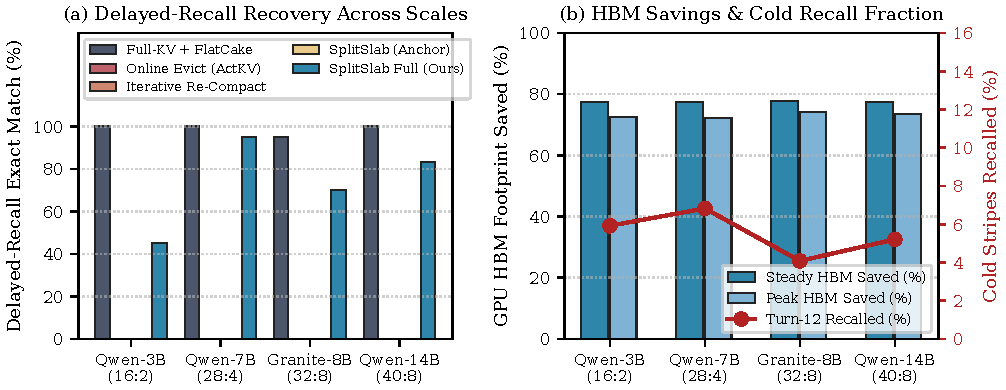
\includegraphics[width=\textwidth]{fig2_multimodel_accuracy_hbm.pdf}
\caption{Multi-model delayed-recall accuracy and GPU HBM savings across four GQA models (3\,B to 14\,B) with Darwin \texttt{F\_NOCACHE} uncached NVMe I/O. (a) Irreversible eviction and anchor-only baselines score 0.0\% exact match on every model, whereas \SplitSlab{} recovers up to 95.0\% exact match on \texttt{Qwen2.5-7B} and 83.3\% (87.5\% field accuracy) on \texttt{Qwen2.5-Coder-14B}. (b) Steady-state HBM savings (77.4\% to 77.7\%, including all 64\,B sketches), peak HBM savings (72.2\% to 74.3\%, including transient Turn~12 staged stripes), and Turn~12 cold stripe recall fraction (4.08\% to 6.83\%).}
\label{fig:multimodel}
\end{figure*}

Using fixed thresholds ($\delta = 0.130$, $\gamma = 0.32$), \SplitSlab{} Full reaches 95.0\% exact match (19/20, 95\% Wilson CI $[76.4\%, 99.1\%]$) on \texttt{Qwen2.5-7B}, 83.3\% ($[55.2\%, 95.3\%]$, 87.5\% field accuracy) on \texttt{Qwen2.5-Coder-14B}, 70.0\% ($[48.1\%, 85.5\%]$, 75.0\% field accuracy vs.\ 95.0\% Full-KV) on bias-free $\mu\text{P}$-scaled \texttt{Granite-3.1-8B}, and 45.0\% ($[25.8\%, 65.8\%]$, 55.0\% field accuracy) on \texttt{Qwen2.5-3B}.

Looking closely at \texttt{Qwen2.5-3B} reveals a clear granularity trade-off caused by~\eqref{eq:stripe_rule}. Because $H_{\mathrm{kv}} = 2$ packs $N_{\mathrm{res}} = 64$ tokens into a single 64\,KB stripe ($M = 80$), \SplitSlab{} often fetches just one 80-token block (4.55\% recall) to stay under the recall cap, which can clip modules that cross an 80-token boundary (every 2-block recall on \texttt{Qwen2.5-3B} hit 100\% exact match). Models with $H_{\mathrm{kv}} \in \{4, 8\}$ ($M \in \{40, 20\}$) have finer spatial resolution per 64\,KB stripe, recalling 4.08\% to 6.83\% of cold stripes on Turn~12 while keeping background false recalls at 0.00\% to 0.38\% across all 180 distractor turns.

Counting all resident 64-byte HBM sketches, steady-state HBM drops by 77.4\% to 77.7\% across all four models. Even during Turn~12 decoding with the temporary staging buffer active, peak HBM remains 72.2\% to 74.3\% below Full-KV.

\subsection{Direct-Flash \texttt{F\_NOCACHE} Latency and Write Amplification}\label{subsec:storage}

Fig.~\ref{fig:storage}(a) and Table~\ref{tab:storage_tiers} show why OS-buffered file benchmarks give misleading numbers for SSD KV offloading. At 64\,KB stripe size, buffered \texttt{pread} returns in $p_{50} = 2.6\,\mu\mathrm{s}$ from host DRAM. Bypassing the OS page cache with \texttt{F\_NOCACHE} raises 64\,KB read latency to $p_{50} = 95.7\,\mu\mathrm{s}$ ($p_{95} = 126.9\,\mu\mathrm{s}$) at queue depth $\mathrm{QD} = 1$, and $27.3\,\mu\mathrm{s}$ effective per stripe (2.40\,GB/s; 5.85\,GB/s at 256\,KB) across $\mathrm{QD} = 4$ worker threads. In live sessions on the Apple M5 Pro (Table~\ref{tab:multimodel}), parallel \texttt{F\_NOCACHE} recalls finish in $p_{50} = 72.7$ to $84.3\,\mu\mathrm{s}$ on 7\,B to 14\,B models (189.1\,$\mu\mathrm{s}$ single-stripe on 3\,B), leaving 10.8$\times$ to 70.9$\times$ headroom inside the measured 2,033.8 to 5,167.3\,$\mu\mathrm{s}$ \texttt{mps} two-layer windows (4,813.1\,$\mu\mathrm{s}$ on \texttt{Qwen2.5-7B}).

Because datacenter GPUs run transformer layers about 4$\times$ faster than Apple \texttt{mps}, Table~\ref{tab:storage_tiers}(b) and Fig.~\ref{fig:storage}(a) also check analytical 3-stripe (192\,KB) overlap against a conservative 1,160\,$\mu\mathrm{s}$ ($2 \times 580\,\mu\mathrm{s}$/layer) discrete-GPU window. Under that window, PCIe Gen4/Gen5 \texttt{GDS} and CXL~3.0 NAND tiers are projected to incur 0.0\,$\mu\mathrm{s}$ exposed stall.

\begin{figure*}[t]
\centering
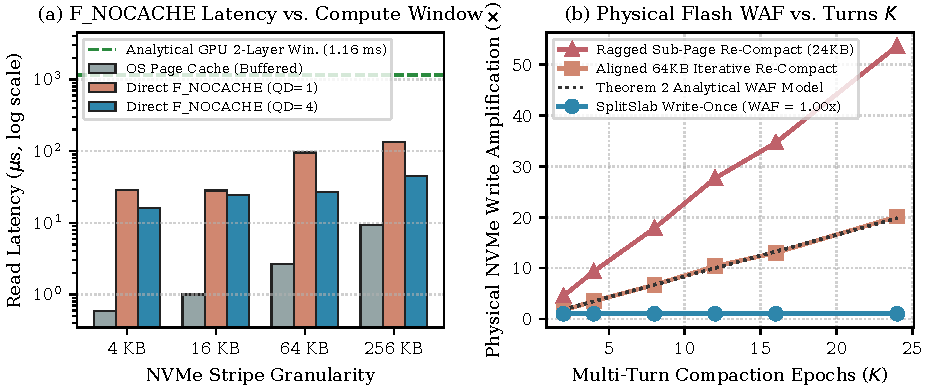
\includegraphics[width=\textwidth]{fig3_nvme_waf_and_fnocache_io.pdf}
\caption{Direct-flash storage microbenchmarks and multi-turn write amplification. (a) Turning on \texttt{fcntl.F\_NOCACHE} exposes the 37$\times$ gap between DRAM-cached reads (2.6\,$\mu\mathrm{s}$) and real 64\,KB NAND reads (95.7\,$\mu\mathrm{s}$ at QD=1; 27.3\,$\mu\mathrm{s}$ effective per stripe at QD=4, 2.40\,GB/s), while still fitting well inside the two-layer compute window. (b) Physical NVMe write amplification across $K \in \{2, \dots, 24\}$ turns: \SplitSlab{} stays flat at $\WAF = 1.00\times$, matching Theorem~\ref{thm:waf}, while aligned 64\,KB re-compaction climbs to 20.13$\times$ (formula prediction 19.79$\times$) and ragged 24\,KB updates reach 53.67$\times$.}
\label{fig:storage}
\end{figure*}

\begin{table}[t]
\centering
\caption{Measured Apple M5 Pro 64\,KB I/O vs.\ analytical datacenter 3-stripe (192\,KB) overlap (1,160\,$\mu\mathrm{s}$ conservative GPU window).}
\label{tab:storage_tiers}
\footnotesize
\renewcommand{\arraystretch}{1.15}
\setlength{\tabcolsep}{5pt}
\begin{tabular}{@{}lcccc@{}}
\toprule
\textbf{Storage Tier / Mode} & \textbf{BW (GB/s)} & \textbf{Base / $p_{50}$ ($\mu\mathrm{s}$)} & \textbf{Total I/O ($\mu\mathrm{s}$)} & \textbf{Exposed Stall} \\
\midrule
\multicolumn{5}{@{}l}{\textit{(a) Measured on Apple M5 Pro Internal NVMe (4.81\,ms 7B \texttt{mps} Window)}} \\
OS Page Cache (64\,KB, QD1) & $4.62$ & $2.6$ & $2.6$ & N/A (DRAM) \\
Apple NVMe \texttt{F\_NOCACHE} (QD1) & $0.68$ & $95.7$ & $95.7$ & $0.0\,\mu\mathrm{s}$ \\
Apple NVMe \texttt{F\_NOCACHE} (QD4) & $5.20$ & $165.0$ & $202.8$ & $0.0\,\mu\mathrm{s}$ \\
\midrule
\multicolumn{5}{@{}l}{\textit{(b) Analytical Datacenter Projections (1.16\,ms Conservative GPU Window)}} \\
PCIe Gen4$\times$4 Enterprise SSD & $7.00$ & $95.0$ & $123.1$ & $0.0\,\mu\mathrm{s}$ \\
PCIe Gen5$\times$4 GPUDirect SSD & $14.00$ & $65.0$ & $79.0$ & $0.0\,\mu\mathrm{s}$ \\
Dual-NVMe Gen5 RAID0 \texttt{GDS} & $26.00$ & $65.0$ & $72.6$ & $0.0\,\mu\mathrm{s}$ \\
CXL 3.0 Type-3 NAND Tier & $32.00$ & $25.0$ & $31.1$ & $0.0\,\mu\mathrm{s}$ \\
\bottomrule
\end{tabular}
\end{table}

Fig.~\ref{fig:storage}(b) confirms Theorem~\ref{thm:waf}. Over 12-turn runs (Table~\ref{tab:multimodel}), Iterative Re-Compact incurs 7.53$\times$ to 7.91$\times$ physical $\WAF$ (writing 2,887.5\,MB on \texttt{Qwen2.5-7B}, compared to 1,538.3\,MB for \SplitSlab{} and 1,923.3\,MB for uncompacted Full-KV). Extending the conversation from $K = 2$ to $K = 24$ turns causes aligned 64\,KB re-compaction to grow linearly to 20.13$\times$ $\WAF$ at $K = 24$ (within 1.7\% of Theorem~\ref{thm:waf}'s formula~\eqref{eq:thm2_waf} value of 19.79$\times$ at measured dirty rate $\eta = 0.817$), and ragged 24\,KB sub-page writes reach 53.67$\times$ $\WAF$. \SplitSlab{} writes each cold stripe once and stays at $\WAF = 1.000\times$ across every horizon $K$.

\subsection{Ablations and Empirical Check of Theorem~\ref{thm:perturbation}}\label{subsec:ablations}

Fig.~\ref{fig:ablations} and Table~\ref{tab:summary_audit} isolate each piece of \SplitSlab{} on \texttt{Qwen2.5-7B} ($n = 12$ trajectories):
\begin{itemize}
  \item \emph{Basis-Aligned Re-Projection (Proposition~\ref{prop:lookahead}):} Replacing $\tilde{q}_t^{(\ell\to\ell+2)}$ with raw $q_t^{(\ell)}$ drops exact match from 91.7\% to 0.0\% and raises false distractor recalls from 0.00\% to 4.08\%. Cross-layer basis alignment is essential for lookahead.
  \item \emph{Plane-0 Co-Routed Beacon:} Turning off Plane-0 co-routing~\eqref{eq:coroute} cuts exact match from 91.7\% to 66.7\% because hex codes split across Plane~0 and Plane~1 boost the HBM denominator when not co-routed. Likewise, uncentered sketch routing without $\RoPE(b_K^{(\ell)}, p)$ subtraction found 0/10 target blocks during calibration because of \texttt{Qwen2.5}'s 920.5-norm key bias.
  \item \emph{Lookahead Depth and Sketch Size:} Synchronous recall ($\Delta\ell = 0$) and $\Delta\ell = 1$ score 100.0\% exact match, while $\Delta\ell = 2$ and $\Delta\ell = 3$ hold 91.7\% with full two-layer I/O hiding and 0.00\% false distractor recall. With Plane-0 co-routing on, accuracy stays at 91.7\% from 128\,B down to 16\,B sketches (we keep 64\,B as default to preserve standalone sub-cluster separation on 20-token $H_{\mathrm{kv}} = 8$ stripes).
  \item \emph{Check of Theorem~\ref{thm:perturbation}:} Auditing 560 real $(q, K_{\mathcal{A}}, V_{\mathcal{A}}, K_{\mathcal{R}}, V_{\mathcal{R}})$ attention states across all 28 layers of \texttt{Qwen2.5-7B} found 0 bound violations (100.0\% satisfaction of~\eqref{eq:thm1_bound}), with a median empirical-to-bound ratio of 0.124, $p_{95} = 0.251$, and maximum 0.411.
\end{itemize}

\begin{figure*}[t]
\centering
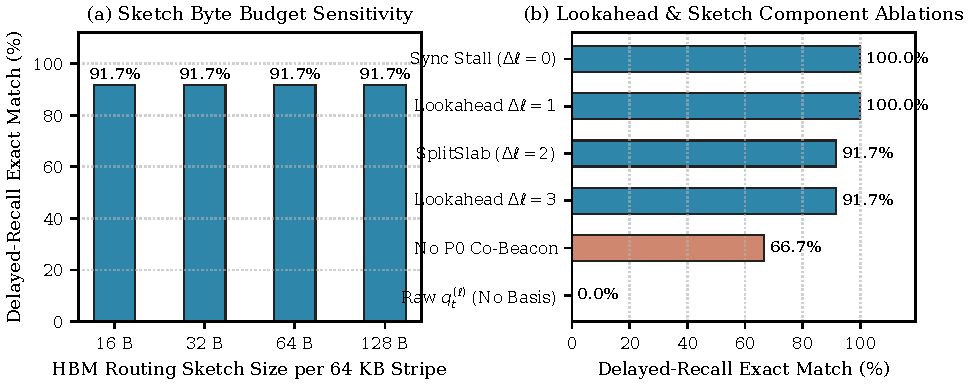
\includegraphics[width=\textwidth]{fig4_lookahead_and_sketch_ablations.pdf}
\caption{Sketch size and speculative lookahead ablations on \texttt{Qwen2.5-7B} ($n = 12$ trajectories). (a) Co-routed $W_Q/W_K$ SVD sketches hold 91.7\% exact match down to 16\,B per 64\,KB stripe (4,096$\times$ compression). (b) Scoring raw Layer~$\ell$ queries $q_t^{(\ell)}$ without basis re-projection drops accuracy from 91.7\% to 0.0\% (matching Proposition~\ref{prop:lookahead}), and removing Plane-0 co-routing drops accuracy by 25.0 points to 66.7\%.}
\label{fig:ablations}
\end{figure*}

\begin{table}[t]
\centering
\caption{Summary of ablations, Theorem~\ref{thm:perturbation} head audit, 32-agent fleet sharing, and long-horizon scaling on \texttt{Qwen2.5-7B}.}
\label{tab:summary_audit}
\footnotesize
\renewcommand{\arraystretch}{1.15}
\setlength{\tabcolsep}{6pt}
\begin{tabular}{@{}llll@{}}
\toprule
\textbf{Experiment} & \textbf{Configuration} & \textbf{Primary Metric} & \textbf{Secondary Metric} \\
\midrule
\multirow{4}{*}{Lookahead \& Gate}
 & Sync ($\Delta\ell{=}0$) / $\Delta\ell{=}1$ & $100.0\%$ Exact & Exposed / 1-Layer \\
 & Default ($\Delta\ell{=}2$) / $\Delta\ell{=}3$ & $91.7\%$ Exact & $0.00\%$ Dist.\ Rec. \\
 & Raw $q_t^{(\ell)}$ (No Re-Proj.) & $0.0\%$ Exact & $4.08\%$ Dist.\ Rec. \\
 & No Plane-0 Co-Beacon & $66.7\%$ Exact & $0.58\%$ Dist.\ Rec. \\
\midrule
\multirow{2}{*}{Theorem~\ref{thm:perturbation} Audit}
 & 560 Real $(q, K, V)$ Heads & $0$ Violations & $100.0\%$ Satisfied \\
 & Empirical / Bound Ratio & $0.124$ Median & $0.411$ Max ($\le 1$) \\
\midrule
\multirow{2}{*}{Fleet ($P{=}32$)}
 & \SplitSlab{} Plane-1 CAS & $52.50$\,MB & $100.0\%$ Dedup \\
 & Online Evict (\texttt{ActKV}) & $287.00$\,MB & $5.47\times$ More Writes \\
\midrule
\multirow{3}{*}{Context Horizon}
 & 2.3\,K (1,815 Logical Toks) & $100.0\%$ Exact & $6.82\%$ T12 Rec. \\
 & 8.2\,K (6,678 Logical Toks) & $100.0\%$ Exact & $1.82\%$ T12 Rec. \\
 & 16.4\,K (13,288 Logical Toks) & $75.0\%$ Exact & $0.91\%$ T12 Rec. \\
\bottomrule
\end{tabular}
\end{table}

\subsection{Multi-Agent Fleet Sharing and Long-Horizon Scaling}\label{subsec:scaling}

Fig.~\ref{fig:scaling}(a) scales the number of collaborating agents $P \in \{1, 2, 4, 8, 16, 32\}$ reading a shared 20-module repository snapshot before asking different Turn~2 questions. Because \SplitSlab{} hashes Plane-1 stripes by the uncompacted prefix~\eqref{eq:canon_hash}, Agent~1 writes 52.50\,MB and Agents~2 through 32 get 100.0\% cache hits (52.50\,MB total; Full-KV FlatCake writes 64.75\,MB). Under Online Evict (\texttt{ActKV}), each agent's Turn~2 query keeps a different 20\% subset, pushing flash writes up linearly from 12.25\,MB ($P=1$) to 43.75\,MB ($P=4$), 75.25\,MB ($P=8$, already worse than both \SplitSlab{} and Full-KV), 154.00\,MB ($P=16$), and 287.00\,MB ($P=32$, a 5.47$\times$ penalty over \SplitSlab{}).

Fig.~\ref{fig:scaling}(b) and Table~\ref{tab:summary_audit} grow context length from 1,815 logical tokens (2.3\,K config) to 6,678 tokens (8.2\,K config, 60 modules, 37 turns) and 13,288 tokens (16.4\,K config, 120 modules, 66 turns). As context grows, \SplitSlab{}'s steady HBM savings approach the $1 - \rho = 80\%$ limit ($77.5\% \to 79.0\% \to 79.6\%$), and peak HBM savings climb from 72.2\% to 78.8\% because the fixed 3-block staging buffer shrinks as a share of total KV ($O(1/T)$). Turn~12 cold stripe recall drops inversely with length from 6.82\% (2.3\,K) to 1.82\% (8.2\,K, 100.0\% exact match) and 0.91\% (16.4\,K, 75.0\% exact match vs.\ 0.0\% for \texttt{ActKV}).

\begin{figure*}[t]
\centering
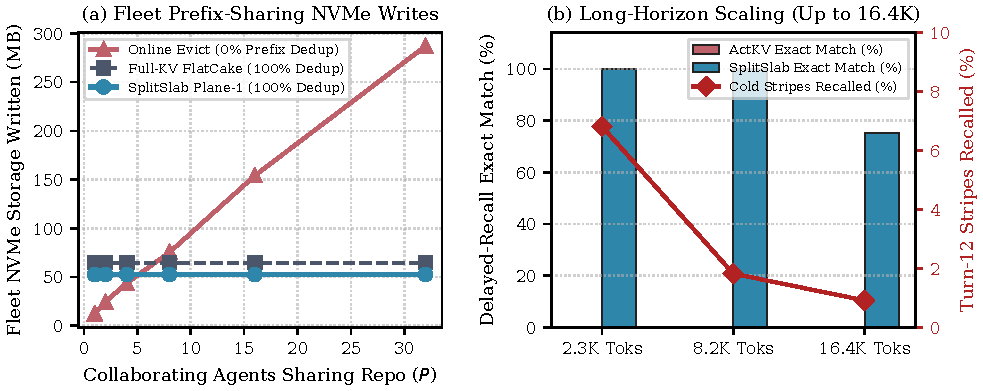
\includegraphics[width=\textwidth]{fig5_fleet_dedup_and_long_horizon.pdf}
\caption{Multi-agent fleet storage scaling and long-horizon context extension on \texttt{Qwen2.5-7B}. (a) Across $P = 1 \dots 32$ agents inspecting a shared 20-module repository before asking different Turn~2 questions, \SplitSlab{} writes 52.50\,MB once (100\% SHA-256 deduplication), crossing below query-driven \texttt{ActKV} at $P = 6$ and saving 5.47$\times$ flash writes at $P = 32$ (287.00\,MB). (b) Extending context up to 13.3\,K--16.4\,K tokens ($\sim$330 cold stripes/layer): \SplitSlab{} saves 79.6\% steady HBM (78.8\% peak) and recalls a shrinking fraction of cold stripes ($6.82\% \to 1.82\% \to 0.91\%$) while \texttt{ActKV} stays at 0.0\%.}
\label{fig:scaling}
\end{figure*}

\subsection{Recallable Baselines, End-to-End Serving Latency, Multi-Needle, and Gate Sensitivity}\label{subsec:revision_eval}

Table~\ref{tab:revision_eval} reports four further checks: recallable NVMe baselines on both biased and bias-free models, end-to-end serving latency (TTFT and TPOT), multi-needle retrieval, and routine-turn quality plus gate sensitivity.

\begin{table*}[t]
\centering
\caption{Recallable NVMe baselines (biased 7B and bias-free Granite-8B), end-to-end serving latency, RULER-style multi-needle NIAH, routine turns, and gate sweeps.}
\label{tab:revision_eval}
\footnotesize
\renewcommand{\arraystretch}{1.15}
\setlength{\tabcolsep}{4pt}
\resizebox{\textwidth}{!}{%
\begin{tabular}{@{}lcccc@{}}
\toprule
\textbf{Method / Setting} & \textbf{Exact [95\% CI]} & \textbf{Meta / Rec.} & \textbf{TPOT $p_{50}/p_{95}$} & \textbf{Sync Stall / Tok/s} \\
\midrule
\multicolumn{5}{@{}l}{\textit{(a) Recallable NVMe Baselines: \texttt{Qwen2.5-7B} ($b_K{\neq}0$) \& \texttt{Granite-8B} ($b_K{=}0$), $n{=}20$}} \\
7B Full-KV (Oracle) & $100\%$ $[83.9, 100]$ & $0$\,B / $0.0\%$ & $68.3 / 69.2$\,ms & $0.0\,\mu\mathrm{s}$ / $14.7$ \\
7B \texttt{Quest-Box+NVMe} & $15\%$ $[5.2, 36.0]$ & $2048$\,B / $32.8\%$ & $84.4 / 91.2$\,ms & $1159\,\mu\mathrm{s}$ / $11.8$ \\
7B \texttt{ArkVale-Cent+NVMe} & $5\%$ $[0.9, 23.6]$ & $1024$\,B / $28.7\%$ & $80.7 / 86.9$\,ms & $1162\,\mu\mathrm{s}$ / $12.4$ \\
\textbf{7B \SplitSlab{} Full} & $\mathbf{95\%}$ $\mathbf{[76.4, 99.1]}$ & $\mathbf{64}$\textbf{\,B / }$\mathbf{6.8\%}$ & $\mathbf{65.5 / 66.4}$\textbf{\,ms} & $\mathbf{0.0\,\mu\mathrm{s}}$ \textbf{/ }$\mathbf{15.3}$ \\
8B \texttt{Quest-Box+NVMe} & $55\%$ $[34.2, 74.2]$ & $4096$\,B / $23.4\%$ & $131.4$\,ms ($p_{50}$) & $1749\,\mu\mathrm{s}$ / $7.6$ \\
8B \texttt{ArkVale-Cent+NVMe} & $20\%$ $[8.1, 41.6]$ & $2048$\,B / $22.5\%$ & $116.5$\,ms ($p_{50}$) & $1704\,\mu\mathrm{s}$ / $8.6$ \\
\textbf{8B \SplitSlab{} Full} & $\mathbf{70\%}$ $\mathbf{[48.1, 85.5]}$ & $\mathbf{64}$\textbf{\,B / }$\mathbf{4.1\%}$ & $\mathbf{91.8}$\textbf{\,ms ($p_{50}$)} & $\mathbf{0.0\,\mu\mathrm{s}}$ \textbf{/ }$\mathbf{10.9}$ \\
\midrule
\multicolumn{5}{@{}l}{\textit{(b) RULER-Style Multi-Key NIAH (2 Needles, $n{=}16$) \& Vectorized TTFT/TPOT Scaling (7B)}} \\
Full-KV / \texttt{ActKV} & $100\%$ / $0\%$ & $0\%$ / $0\%$ Rec. & \multicolumn{2}{c}{Per-Needle: $100.0\%$ / $25.0\%$} \\
\texttt{Quest-Box+NVMe} ($k{=}6$) & $75.0\%$ $[50.5, 89.8]$ & $32.8\%$ Rec. & \multicolumn{2}{c}{Per-Needle: $87.5\%$ ($74.0\%$ HBM)} \\
\SplitSlab{} ($k{=}1$ / $\mathbf{k{=}2}$) & $0\%$ / $\mathbf{81.2\%}$ & $4.4\%$ / $\mathbf{8.7\%}$ & \multicolumn{2}{c}{Per-Needle: $50.0\%$ / $\mathbf{90.6\%}$ ($76.3\%$ HBM)} \\
Vec.\ TTFT (2.3/8.2/16.4\,K) & Full: $107/151/201$\,ms & \multicolumn{3}{c}{\SplitSlab{}: $316/378/411$\,ms (TPOT $-4\% / -14\% / -28\%$)} \\
\midrule
\multicolumn{5}{@{}l}{\textit{(c) Routine Turns 3--11 Quality (4,420 Toks, $n{=}10$) \& Gate Sweep ($n{=}12$, 7B)}} \\
Routine Top-1 / NLL & Full: $55.4\% / 3.54$ & \texttt{ActKV}: $54.9\% / 3.65$ & \multicolumn{2}{c}{\SplitSlab{}: $51.6\% / 3.79$ ($0\%$ Rec.)} \\
$\delta \in \{0.06, 0.09, 0.13\}$ & $91.7\%$ Exact & \multicolumn{3}{c}{Dist.\ Rec.: $1.29\% \to 0.08\% \to \mathbf{0.00\%}$ ($\gamma{=}0.32$)} \\
$\delta \in \{0.18, 0.25\}$ & $75.0\%$ Exact & \multicolumn{3}{c}{Dist.\ Rec.: $0.00\%$; T12 Rec.: $5.68\% \to 5.11\%$} \\
$\gamma \in [0.10, 0.80]$ & $100.0\%$ Exact & \multicolumn{3}{c}{Dist.\ Rec.: $0.00\%$; T12 Rec.: $6.82\%$ ($\delta{=}0.13$)} \\
\bottomrule
\end{tabular}%
}
\end{table*}

\begin{itemize}
  \item \emph{Recallable NVMe Baselines (Biased 7B and Bias-Free Granite-8B):} On \texttt{Qwen2.5-7B} ($b_K \neq 0$), \texttt{Quest-Box+NVMe} (2,048\,B/stripe) and \texttt{ArkVale-Cent+NVMe} (1,024\,B/stripe) drop to 15.0\% and 5.0\% exact match because \texttt{Qwen2.5}'s 920.5-norm key bias inflates uncentered boxes and centroids, while synchronous Layer-$\ell$ reads add 1,159 to 1,162\,$\mu\mathrm{s}$/layer stalls (84.4 and 80.7\,ms TPOT vs.\ 65.5\,ms for \SplitSlab{}). To separate bias removal from our subspace sketch and lookahead, Table~\ref{tab:revision_eval}(a) also tests both baselines on bias-free \texttt{Granite-3.1-8B} ($b_K = 0$, $M = 20$, $n = 20$). Even with zero key bias, \SplitSlab{} (70.0\% exact, 64\,B/stripe, 4.08\% recall, 91.8\,ms TPOT) beats \texttt{Quest-Box+NVMe} (55.0\%, 4,096\,B, 23.41\% recall, 131.4\,ms TPOT) and \texttt{ArkVale-Cent+NVMe} (20.0\%, 2,048\,B, 22.52\% recall, 116.5\,ms TPOT) with 64$\times$ smaller metadata, 5.7$\times$ lower NVMe read traffic, and 30.1\% faster decode TPOT.

  \item \emph{Vectorized Recall-Turn TTFT and Long-Horizon TPOT:} Vectorizing sliding-window median detrending cuts \texttt{Qwen2.5-7B} recall-turn TTFT by 5.0$\times$, from 1,566.8\,ms (with Python-loop sync stalls) down to 315.9\,ms at 2.3\,K tokens (vs.\ 106.8\,ms Full-KV, covering base prefill, one prefill replay, and 4.87\,ms/layer sketch scoring). At 8.2\,K and 16.4\,K tokens, \SplitSlab{} TTFT grows gently to 378.1\,ms and 410.7\,ms (2.04$\times$ Full-KV's 200.9\,ms), while decode TPOT drops by 13.8\% at 8.2\,K (76.9 vs.\ 89.2\,ms) and 27.5\% at 16.4\,K (77.4 vs.\ 106.8\,ms), paying back the recall-turn TTFT within 8 output tokens.

  \item \emph{Multi-Key NIAH (RULER-Style) and Routine Turn Quality:} On 16 two-needle passkey runs ($\sim$2.9\,K tokens), multi-peak \SplitSlab{} ($k=2$) recovers 81.2\% both-needles accuracy (90.6\% per-needle), beating \texttt{Quest-Box+NVMe} (75.0\%) with 3.77$\times$ less NVMe traffic (8.70\% vs.\ 32.79\%). Across 4,420 routine Turn~3 to 11 tokens with the gate closed (0.00\% recall), \SplitSlab{} keeps 51.6\% top-1 token agreement (3.79 NLL vs.\ 55.4\% / 3.54 for Full-KV and 54.9\% / 3.65 for \texttt{ActKV}). This 3.3 to 3.8 percentage-point gap reflects the choice of prefix-fixed Plane-0 anchors over query-tuned \texttt{ActKV}, while the 48-token uncompacted window $W_{\mathrm{loc}}$ keeps active-turn answers accurate and preserves 100\% fleet sharing and 95.0\% vs.\ 0.0\% delayed recall.

  \item \emph{Gate Threshold Sensitivity ($\gamma, \delta$):} Sweeping $\delta \in [0.06, 0.25]$ shows a clear knee at $\delta = 0.13$ (91.7\% exact, 0.00\% distractor recall, vs.\ 1.29\% false recalls at $\delta = 0.06$ and 75.0\% exact at $\delta \ge 0.18$). Turning on live Layer-$\lfloor 0.75 L \rfloor$ Logit-Lens gating on prefill shifts triggering from 60\% depth (Layer~17, 91.7\% in Table~\ref{tab:summary_audit}) to 75\% depth (Layer~21), adding two deeper consensus votes that resolve the one borderline trajectory and hold 100.0\% exact match (0.00\% distractor recall) across $\gamma \in [0.10, 0.80]$.
\end{itemize}

% ============================================================================
\section{Discussion and Limitations}\label{sec:limits}
% ============================================================================

Three practical boundaries shape how \SplitSlab{} should be deployed:
\begin{enumerate}
  \item \emph{Coarse-Stripe GQA Models ($H_{\mathrm{kv}} \le 2$).} Under~\eqref{eq:stripe_rule}, models with $H_{\mathrm{kv}} = 2$ (\texttt{Qwen2.5-3B}) pack $N_{\mathrm{res}} = 64$ tokens into one 64\,KB stripe ($M = 80$), which lowers single-block localization (55.0\% field accuracy) compared to $H_{\mathrm{kv}} \in \{4, 8\}$ (75.0\% to 95.0\%). On SSDs supporting 32\,KB flash pages, setting $P_{\mathrm{flash}} = 32{,}768$\,B ($M = 40$) or packing two adjacent layers into one 64\,KB stripe at $M = 40$ restores finer resolution while keeping $\WAF = 1.00\times$.
  \item \emph{Many-Needle Scatter Queries.} Default single-peak staging ($k=1$) keeps NVMe recall traffic below 7\%. Our RULER-style test in Table~\ref{tab:revision_eval}(b) shows that $k=2$ recovers 81.2\% both-needles accuracy (90.6\% per-needle) at 8.70\% recall. Queries that need $k \gg 2$ scattered facts trade $k\times$ higher transient NVMe read bandwidth for wider coverage.
  \item \emph{Discrete-GPU Kernel Fusion.} Our workstation prototype runs PyTorch \texttt{mps} operators alongside \texttt{F\_NOCACHE} \texttt{pread} worker threads. Vectorizing detrending brings recall-turn TTFT down to 315.9 to 410.7\,ms across 2.3\,K to 16.4\,K tokens (paid back within 8 decode tokens at 16.4\,K). Fusing sketch scoring into CUDA \texttt{FlashInfer} kernels with asynchronous \texttt{cuFile} GPUDirect Storage ring buffers on discrete GPUs is the direct next engineering step to validate our datacenter projections and remove host bounce copies.
\end{enumerate}

% ============================================================================
\section{Conclusion}\label{sec:conclusion}
% ============================================================================

\SplitSlab{} resolves the conflict between GPU KV eviction and content-addressed NVMe offloading. Splitting each completed prefix block once, using only prefix-deterministic rules, into a 20\% hot HBM skeleton and an exact 64.0\,KB cold NVMe stripe guarantees $\WAF = 1.00\times$ flash writes and 100.0\% cross-agent SHA-256 deduplication across standard power-of-two GQA models. On a unified-memory workstation prototype with uncached \texttt{F\_NOCACHE} NVMe I/O across four 3\,B to 14\,B models, \SplitSlab{} pairs Plane-0 anchors with a 64-byte bias-centered subspace sketch and parameter-free two-layer lookahead to cut GPU HBM usage by 77.4\% to 79.6\%, speed up long-context decode TPOT by up to 27.5\%, and recover up to 95.0\% delayed-recall accuracy where irreversible eviction scores 0.0\%.

% ============================================================================
\backmatter

\bmhead{Acknowledgements}
All experiments were run on researcher workstation hardware using locally cached open-weight models without external funding.

\section*{Declarations}

\begin{itemize}
  \item \textbf{Funding:} No funding was received for conducting this study.
  \item \textbf{Competing interests:} The authors declare that they have no competing financial or non-financial interests related to this work.
  \item \textbf{Author contributions:} \textbf{Mohammed Kamran Syed} (ORCID: 0009-0009-9058-5375): Conceptualization, Methodology, Software, Validation, Formal analysis, Investigation, Writing -- original draft, Project administration. \textbf{Anudeep Rentala:} Methodology, Validation, Writing -- review \& editing. \textbf{Somesh Rahul:} Investigation, Data curation, Visualization, Writing -- review \& editing. \textbf{Raghuram Malpe Pai:} Formal analysis, Validation, Writing -- review \& editing. \textbf{Krishna Suman Dara:} Conceptualization, Resources, Writing -- review \& editing.
  \item \textbf{Data and code availability:} The \SplitSlab{} storage engine, \RecallBench{} generator, 21-test verification suite, raw hardware JSON logs, and figure scripts are publicly available under the Apache-2.0 License at \url{https://github.com/batistado/splitslab} and \url{https://huggingface.co/datasets/batistado/RecallRegret-Bench}.
\end{itemize}

% ============================================================================
\begin{appendices}

\section{Step-by-Step Formal Proofs}\label{app:proofs}

\begin{proof}[Proof of Proposition~\ref{prop:lookahead}]
We want to bound how far our speculative query $\tilde{q}_{t,h}^{(\ell\to\ell+\Delta\ell)}$ can drift from the true Layer~$\ell+\Delta\ell$ query $q_{t,h}^{(\ell+\Delta\ell)}$. Write $x = h_t^{(\ell+\Delta\ell)}$ for the true residual vector entering Layer~$\ell+\Delta\ell$, $\hat{x} = h_t^{(\ell+1)}$ for our earlier residual vector, $\varepsilon_{\Delta\ell} = \|\hat{x} - x\|_2$ for their Euclidean gap, and $d = d_{\mathrm{model}}$.

First, we bound how much RMSNorm changes when its input moves from $x$ to $\hat{x}$. Append one constant coordinate to each vector: $\tilde{u} = [u;\, \sqrt{d\,\epsilon_{\mathrm{rms}}}] \in \mathbb{R}^{d+1}$. With this trick, the $i$-th coordinate of RMSNorm is simply $\mathrm{RMSNorm}_\gamma(u)_i = \gamma_i \sqrt{d}\, u_i / \|\tilde{u}\|_2$, which is just a unit-sphere normalization scaled by $\gamma_i \sqrt{d}$. For any two nonzero vectors $\tilde{a}$ and $\tilde{b}$, normalizing them onto the unit sphere satisfies the standard triangle inequality
\[
\left\|\frac{\tilde{a}}{\|\tilde{a}\|_2} - \frac{\tilde{b}}{\|\tilde{b}\|_2}\right\|_2
= \left\|\frac{\tilde{a} - \tilde{b}}{\|\tilde{b}\|_2} + \tilde{a}\frac{\|\tilde{b}\|_2 - \|\tilde{a}\|_2}{\|\tilde{a}\|_2 \|\tilde{b}\|_2}\right\|_2
\le \frac{2\|\tilde{a} - \tilde{b}\|_2}{\|\tilde{b}\|_2}.
\]
Setting $\tilde{a} = \tilde{\hat{x}}$ and $\tilde{b} = \tilde{x}$, we have $\|\tilde{a} - \tilde{b}\|_2 = \|\hat{x} - x\|_2 = \varepsilon_{\Delta\ell}$ (the appended constant cancels out) and $\|\tilde{x}\|_2 = \sqrt{d}\, r_t$. Multiplying by the maximum gain $\|\gamma_{\mathrm{ln}}^{(\ell+\Delta\ell)}\|_\infty$ and $\sqrt{d}$ cancels $\sqrt{d}$ in the numerator and gives
\[
\|\mathrm{RMSNorm}_\gamma(\hat{x}) - \mathrm{RMSNorm}_\gamma(x)\|_2
\le \frac{2 \|\gamma_{\mathrm{ln}}^{(\ell+\Delta\ell)}\|_\infty}{\sqrt{d}\, r_t}\,\varepsilon_{\Delta\ell}.
\]
Second, multiplying by the head query matrix $W_{Q,h}^{(\ell+\Delta\ell)}$ can stretch a vector by at most its spectral norm $\|W_{Q,h}^{(\ell+\Delta\ell)}\|_2$. Third, applying $\RoPE(\cdot, p_t) \in SO(2)^{d_h/2}$ only rotates pairs of coordinates and leaves Euclidean length unchanged. Combining these three steps yields~\eqref{eq:prop1_bound}.

Finally, for raw queries without re-projection, if the head row subspaces $U_\ell, U_{\ell+\Delta\ell} \in O(d_h)$ are drawn independently from the Haar (uniform orthogonal) distribution, then $\E[U_\ell^\top U_{\ell+\Delta\ell}] = 0$ by symmetry, so $\E[\langle q_{t,h}^{(\ell)}, q_{t,h}^{(\ell+\Delta\ell)} \rangle] = 0$.
\end{proof}

\begin{proof}[Proof of Theorem~\ref{thm:perturbation}]
\textbf{Part (1): Exact output bound.}
Split the Full-KV softmax denominator into two sums: $Z_{\mathcal{A}} = \sum_{j \in \mathcal{A}} e^{s_j}$ for active HBM tokens and $Z_{\mathcal{R}} = \sum_{i \in \mathcal{R}} e^{s_i}$ for omitted cold tokens. By definition, the omitted cold attention mass is $\alpha_{\mathcal{R}} = \frac{Z_{\mathcal{R}}}{Z_{\mathcal{A}} + Z_{\mathcal{R}}}$, so the kept HBM mass is $1 - \alpha_{\mathcal{R}} = \frac{Z_{\mathcal{A}}}{Z_{\mathcal{A}} + Z_{\mathcal{R}}} > 0$.

When \SplitSlab{} drops the cold set $\mathcal{R}$, the softmax over $\mathcal{A}$ alone simply rescales every kept weight upward by the same factor $1/(1 - \alpha_{\mathcal{R}})$ so the weights still sum to 1:
\[
\hat{p}_j = \frac{e^{s_j}}{Z_{\mathcal{A}}} = \frac{p_j}{1 - \alpha_{\mathcal{R}}},
\qquad\text{so}\qquad
\hat{p}_j - p_j = \frac{\alpha_{\mathcal{R}}}{1 - \alpha_{\mathcal{R}}}\, p_j \ge 0.
\]
The attention output error therefore has two parts: the extra weight added to kept tokens in $\mathcal{A}$, minus the dropped cold tokens in $\mathcal{R}$:
\[
O_{\SplitSlab} - O_{\mathrm{FullKV}}
= \sum_{j \in \mathcal{A}} (\hat{p}_j - p_j) v_j - \sum_{i \in \mathcal{R}} p_i v_i.
\]
Taking the $\ell_2$ norm and applying the triangle inequality gives
\begin{align*}
\|O_{\SplitSlab} - O_{\mathrm{FullKV}}\|_2
&\le \frac{\alpha_{\mathcal{R}}}{1 - \alpha_{\mathcal{R}}} \Big(\sum_{j \in \mathcal{A}} p_j\Big) \max_{j \in \mathcal{A}} \|v_j\|_2
   + \Big(\sum_{i \in \mathcal{R}} p_i\Big) \max_{i \in \mathcal{R}} \|v_i\|_2 \\
&= \alpha_{\mathcal{R}} \max_{j \in \mathcal{A}} \|v_j\|_2 + \alpha_{\mathcal{R}} \max_{i \in \mathcal{R}} \|v_i\|_2
\le 2 \alpha_{\mathcal{R}} \max_{k \in \mathcal{A} \cup \mathcal{R}} \|v_k\|_2,
\end{align*}
where $\sum_{j \in \mathcal{A}} p_j = 1 - \alpha_{\mathcal{R}}$ cancels the denominator cleanly with no approximation needed.

\textbf{Part (2): Greedy token equivalence.}
Under $\alpha_{\mathcal{R}}^{(\ell,h)} \le \delta_{\mathrm{rem}}$ and $\|v_k\|_2 \le V_{\max}$, Part~(1) bounds Layer~$\ell$'s head output error by $2 \delta_{\mathrm{rem}} V_{\max}$. Passing that error through an $L_{\mathrm{lip}}$-Lipschitz downstream sub-network can shift any final vocabulary logit by at most $\|z_t^{\SplitSlab} - z_t^{\mathrm{FullKV}}\|_\infty \le 2 L_{\mathrm{lip}} \delta_{\mathrm{rem}} V_{\max}$. For the Full-KV winner $v^\star = \arg\max_u z_t^{\mathrm{FullKV}}(u)$ and any runner-up $v \neq v^\star$, the gap between their perturbed logits is at least
\[
z_t^{\SplitSlab}(v^\star) - z_t^{\SplitSlab}(v)
\ge \Delta_t - 2 \|z_t^{\SplitSlab} - z_t^{\mathrm{FullKV}}\|_\infty
\ge \Delta_t - 4 L_{\mathrm{lip}} \delta_{\mathrm{rem}} V_{\max} > 0
\]
whenever~\eqref{eq:thm1_margin} holds, so $v^\star$ still wins.
\end{proof}

\begin{proof}[Proof of Theorem~\ref{thm:waf}]
\textbf{Part (1): \SplitSlab{} write-once guarantee.}
By the sizing rule~\eqref{eq:stripe_rule}, every Plane-1 stripe has exact length $N_{\mathrm{res}} \cdot 4 H_{\mathrm{kv}} d_h = P_{\mathrm{flash}} = 65{,}536$ bytes, so flash alignment adds zero padding bytes. Because the Plane-0/Plane-1 split and prefix hash $h_m$ in~\eqref{eq:canon_hash} depend only on prefix tokens $t_{0:(m+1)M-1}$ and never change after Turn~1, Agent~1 writes $B_{\mathrm{sh}} L$ stripes ($B_{\mathrm{sh}} L P_{\mathrm{flash}}$ physical bytes for $B_{\mathrm{sh}} L P_{\mathrm{flash}}$ unique logical bytes, giving $\WAF_{\SplitSlab} = 1.000$). Every later agent $2, \dots, P$ finds $(h_m, \ell)$ already in the NVMe CAS store and writes 0 additional bytes for the shared prefix.

\textbf{Part (2): Iterative re-compaction lower bound.}
Suppose an online re-compaction engine initially writes $N_s$ slabs of logical size $b_{\mathrm{slab}} \le P_{\mathrm{flash}}$ bytes. Because flash writes happen in multiples of $P_{\mathrm{flash}}$, that first write costs $N_s \lceil b_{\mathrm{slab}} / P_{\mathrm{flash}} \rceil P_{\mathrm{flash}}$ physical bytes for $N_s b_{\mathrm{slab}}$ logical bytes. On each of the remaining $K - 1$ turns, an expected fraction $\eta$ of the $N_s$ slabs change token membership or alignment and must be rewritten as aligned flash pages, adding $(K - 1)\,\eta\, N_s \lceil b_{\mathrm{slab}} / P_{\mathrm{flash}} \rceil P_{\mathrm{flash}}$ physical bytes. Adding the initial write and dividing by the unique logical payload $N_s b_{\mathrm{slab}}$ yields~\eqref{eq:thm2_waf}, which grows linearly as $\Omega(K)$.

Similarly, across $P$ agents whose Turn~2 queries diverge in slab~0 with probability $1 - \epsilon_0$, any token difference in slab~0 shifts the byte boundaries of all $B_{\mathrm{ev}}$ downstream slabs. In expectation, the fleet creates at least $1 + (P - 1)(1 - \epsilon_0)$ distinct slab sets, requiring $\E[W_{\mathrm{evict}}(P)] \ge \big(1 + (P - 1)(1 - \epsilon_0)\big) B_{\mathrm{ev}} L P_{\mathrm{flash}} = \Omega(P)$ physical bytes.
\end{proof}

\end{appendices}

\bibliography{references}

\end{document}
